\chapter{Role of Astrophysical Modeling on Dark Matter Halo Relaxation Response at Redshifts $z=0$ and $z=1$}
\label{chap:physvar_z01}

Advancements in computational cosmology have produced state-of-the-art hydrodynamical simulations of cosmological volumes with realistic galaxies (see, e.g., OWLS \citep{2010MNRAS.402.1536S}, Illustris \citep{2014MNRAS.445..175G}, FIRE \citep{2014MNRAS.445..581H}, EAGLE \citep{2015MNRAS.446..521S}, Horizon-AGN \citep[][]{2017MNRAS.467.4739K}, SIMBA \citep[][]{2019MNRAS.486.2827D}, IllustrisTNG \citep{2019ComAC...6....2N}). However, many sub-galactic astrophysical processes, such as star formation, are not resolved by these simulations. Instead, they rely on subgrid prescriptions with parameters calibrated to a set of empirical observations. Ambiguities in the modeling and the calibrated quantities have led to inconsistent results. Additionally, these simulations are computationally expensive to perform, which is why dark matter haloes have typically been studied using gravity-only simulations. Nevertheless, the impact of baryonic processes on the dark matter can be significant and must be accounted for before comparing against observations.

Early studies of individual haloes modeled the response of the radial distribution of dark matter to galaxy formation as adiabatic relaxation \citep[][]{osti6457593,1984MNRAS.211..753B,1986ApJ...301...27B,1987ApJ...318...15R}. However, this idealistic model rarely predicts the dark matter distribution within haloes in hydrodynamical cosmological simulations \citep[e.g.,][]{2004ApJ...616...16G,2010MNRAS.407..435A}. Moreover, the halo response was found to vary widely across haloes and in different simulations \citep[][]{2004ApJ...616...16G,2006PhRvD..74l3522G,2010MNRAS.402..776P,2010MNRAS.406..922T,2010MNRAS.405.2161D,2010MNRAS.407..435A,2011MNRAS.414..195T,2016MNRAS.461.2658D,2019A&A...622A.197A,2022MNRAS.511.3910F,2023Velmani&Paranjape}, leading to the development of various models of the response, some of which are direct extensions of adiabatic relaxation \citep[e.g.,][]{2004ApJ...616...16G,2006PhRvD..74l3522G,2010MNRAS.407..435A}.

In \chapref{chap:z0_main}, we have demonstrated that introducing an additional dependence on the halo-centric distance makes the relation between $r_f/r_i$ and $M_i/M_f$ linear across a variety of haloes in both IllustrisTNG and EAGLE simulations at the present epoch ($z=0$). Based on those results, we have presented a simple prescription for computing the relaxed dark matter mass profiles. In the first part of this chapter, we investigate if such a relaxation model can also be used at an earlier redshift.

Previous works have shown that feedback from various galactic processes strongly influences halo relaxation \citep{2011MNRAS.414..195T}. These effects primarily affect the offset in the relaxation relation, quantifying the excess relaxation experienced by the dark matter \citep{2023Velmani&Paranjape}. We have argued in \chapref{chap:z0_main}, that this could be the reason for the small deviations in the relaxation offset across haloes with different star formation activities. In this chapter, we systematically the role of various astrophysical processes in the galaxy, such as feedback, in mediating the relaxation response of the halo using simulations with variations in the feedback implementation.

This chapter is organized as follows. In \secref{sec:res-itng-z01}, we explore the relaxation response at an earlier redshift in the IllustrisTNG reference simulation. This allows us to understand how the different galactic processes occurring at earlier times affect dark matter halo relaxation. Then in \secref{sec:res-physvar-CAMELS}, we systematically study the relaxation response as a function of the feedback related parameters in the IllustrisTNG model using the set of simulations from CAMELS as described in \secref{sec:sims-CAMELS}. 
Following this, we investigate the role of a variety of astrophysical processes in the EAGLE physics variation simulations described in \secref{sec:sims-EAGLE} and conclude in \secref{sec:conclusion-ch:physvar}.

\section{Early epoch in IllustrisTNG simulations}
\label{sec:res-itng-z01}

In this section, we investigate the relaxation response in the radial distribution of dark matter in the main simulations of IllustrisTNG simulations at an earlier redshift of $z = 1$ and compare it to the present redshift of $z = 0$. Haloes at both these redshifts were identified and matched between hydrodynamical and the corresponding gravity-only runs as described in \secref{sec:hals}. Additionally, we use the SubLink merger tree catalogues to trace the most massive progenitor haloes at $z=1$ of the haloes considered at $z=0$. While present epoch haloes are sampled only by their masses at the present time, we consider three different methods for sampling the early epoch haloes. This results in four distinct sets of halo samples:

\begin{enumerate}
    \item $z=1$ haloes sampled by their masses at $z=1$.
    \item $z=1$ haloes sampled by the masses of their descendants at $z=0$. Note that not all haloes with a given mass at the present time have valid progenitors with the same mass at $z=1$.
    \item $z=1$ haloes sampled by their masses at $z=1$, but the mass bins are defined by the median masses of the most massive progenitors of the $z=0$ haloes.
    \item $z=0$ haloes sampled by their masses at $z=0$.
\end{enumerate}

In each case, the mass bins are defined as described in \secref{sec:results-mass-ch:z0main} considering the mass of the gravity-only halo. The representative colors to represent this halo mass is shown in \figref{fig:mass_bin_label-z01}. Additionally, this figure indicates the peak heights ($\nu$) corresponding to these halo masses at both $z=0$ and $z=1$. These values correspond to the rarity of haloes with that mass at that redshift with rarer haloes having larger values of $\nu$. This can be used to identify mass of the halo at $z=1$ that will have same rarity as $z=0$ halo of a given mass. 

For each of these four sets of halo samples, the average relaxation relations ($r_f/r_i$ vs $M_i/M_f$) are shown in \figref{fig:fit-view-mass-indep}. The bottom right panel, reproduces the \figref{fig:fit-view-mass-indep-ch:z0main} and shown here for comparison. We find that, for a given halo mass, relaxation is usually stronger at the earlier epoch (top left panel) compared to the present time $z=0$ (bottom right panel). In both cases, the trend in relaxation with halo mass is similar, with the strongest relaxation observed in $10^{12} \Mh$ haloes. Interestingly, cluster-scale haloes with masses of $10^{14} \Mh$ at redshift $z=1$ exhibit significant relaxation, unlike clusters of similar size at the present time.

The progenitors at redshift $z=1$ of the same haloes found at $z=0$ show even stronger relaxation, especially in Milky Way-scale and larger haloes, as shown in the top right panel of \figref{fig:fit-view-mass-indep}. The relaxation follows the simple quasi-adiabatic model \eqref{eq:chi-linear-ch:sims} with $q=0.33$ among larger cluster-scale ($10^{14} \Mh$) haloes, while group-scale haloes are consistent with the second-order polynomial relation proposed by Abadi et al. (2010) \cite{2010MNRAS.407..435A}. In the bottom left panel, the relaxation relation is shown for all haloes within a narrow mass bin around the median mass of the progenitors of the haloes selected at $z=0$. Notice that the relaxation relation shifts further lower in Milky Way-scale haloes and smaller clusters with the inclusion of those additional haloes.

\begin{figure}[htbp]
\centering
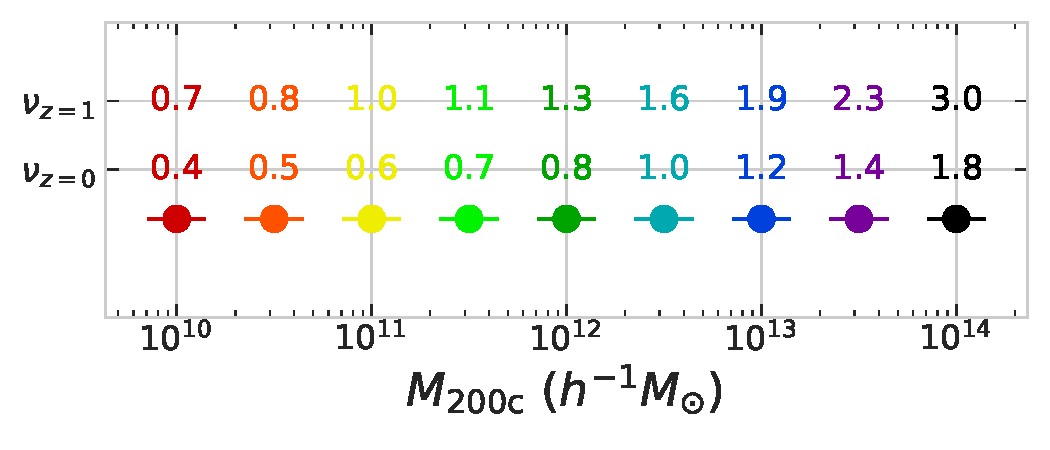
\includegraphics[width=0.49\linewidth]{plots/Mass_bin_labels_z.pdf}
\caption{Representative colors denoting each of the halo mass bins. The numbers in the figure indicate the corresponding values of peak heights $\nu$ at redshifts $z=0$ and $z=1$.}
\label{fig:mass_bin_label-z01}
\end{figure}

\begin{figure*}
\centering
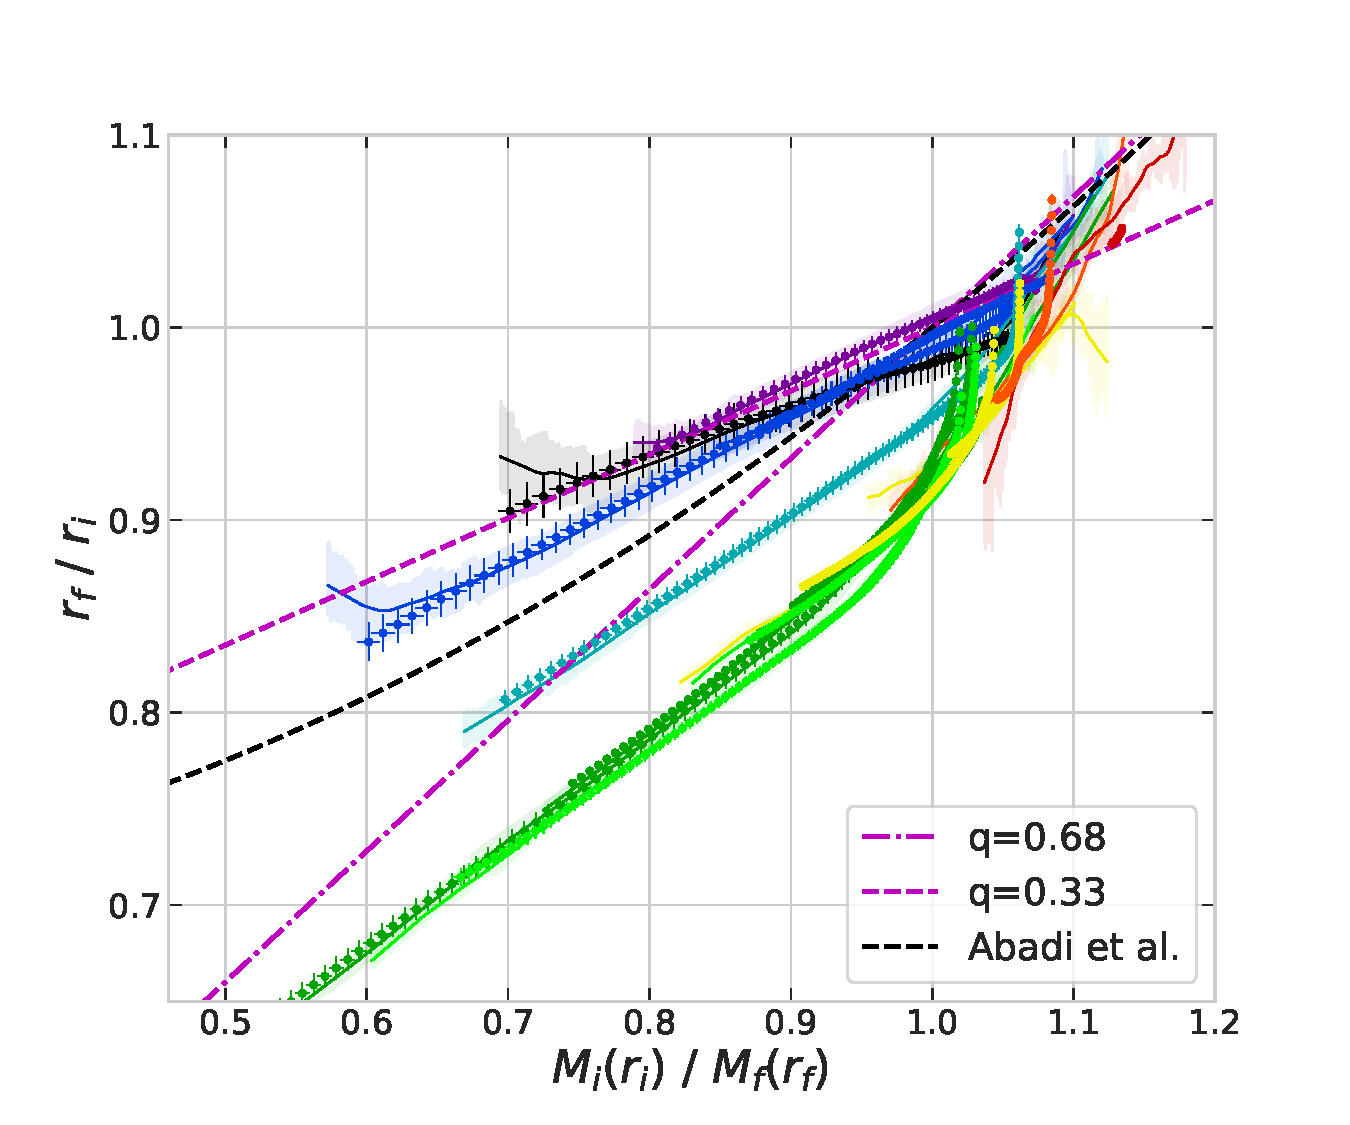
\includegraphics[width=0.48\linewidth]{plots/fit_view_M_T_snap049.pdf}
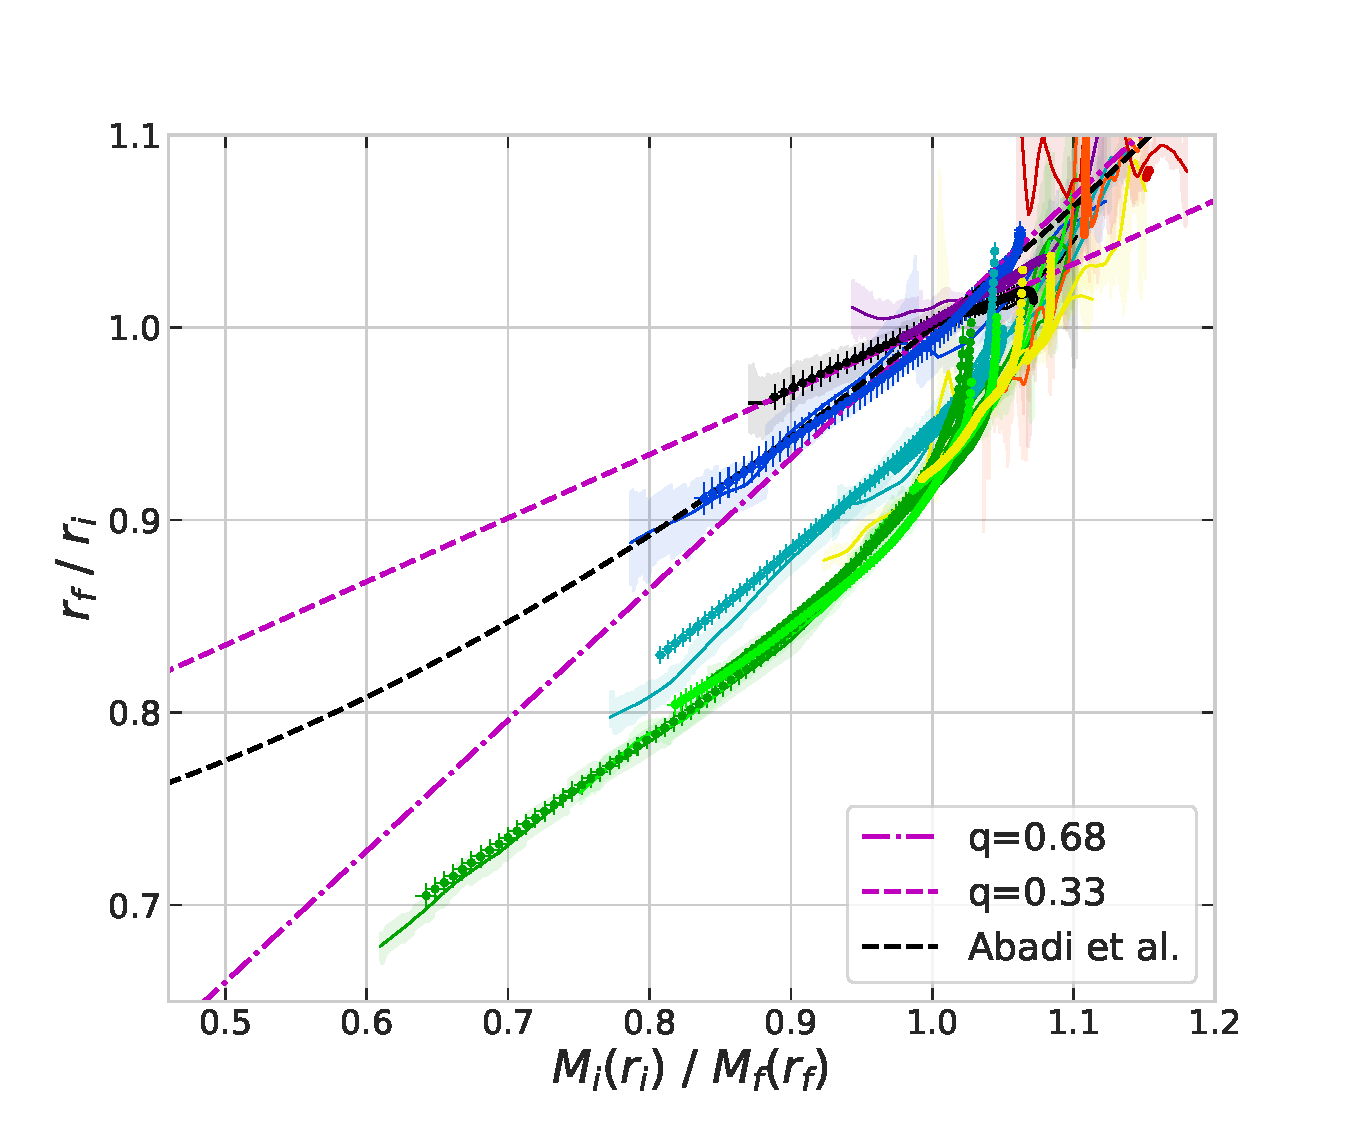
\includegraphics[width=0.48\linewidth]{plots/fit_view_M_T_snap049_smpl98.pdf}
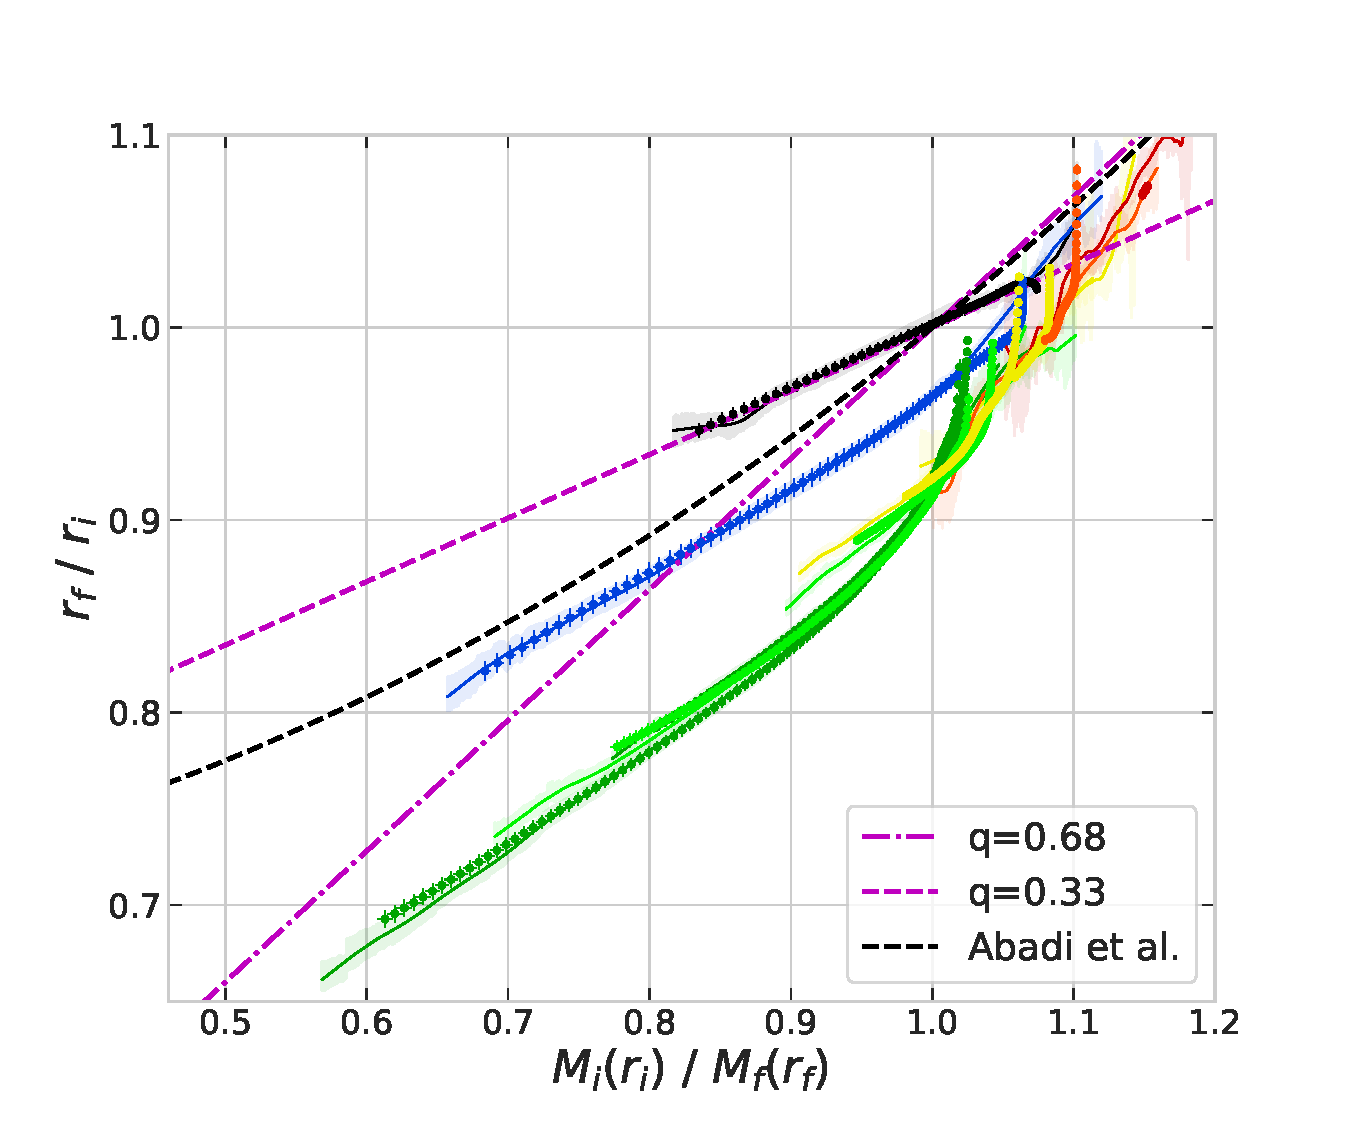
\includegraphics[width=0.48\linewidth]{plots/fit_view_M_T_snap049_smpl98_allHalsMrange.pdf}
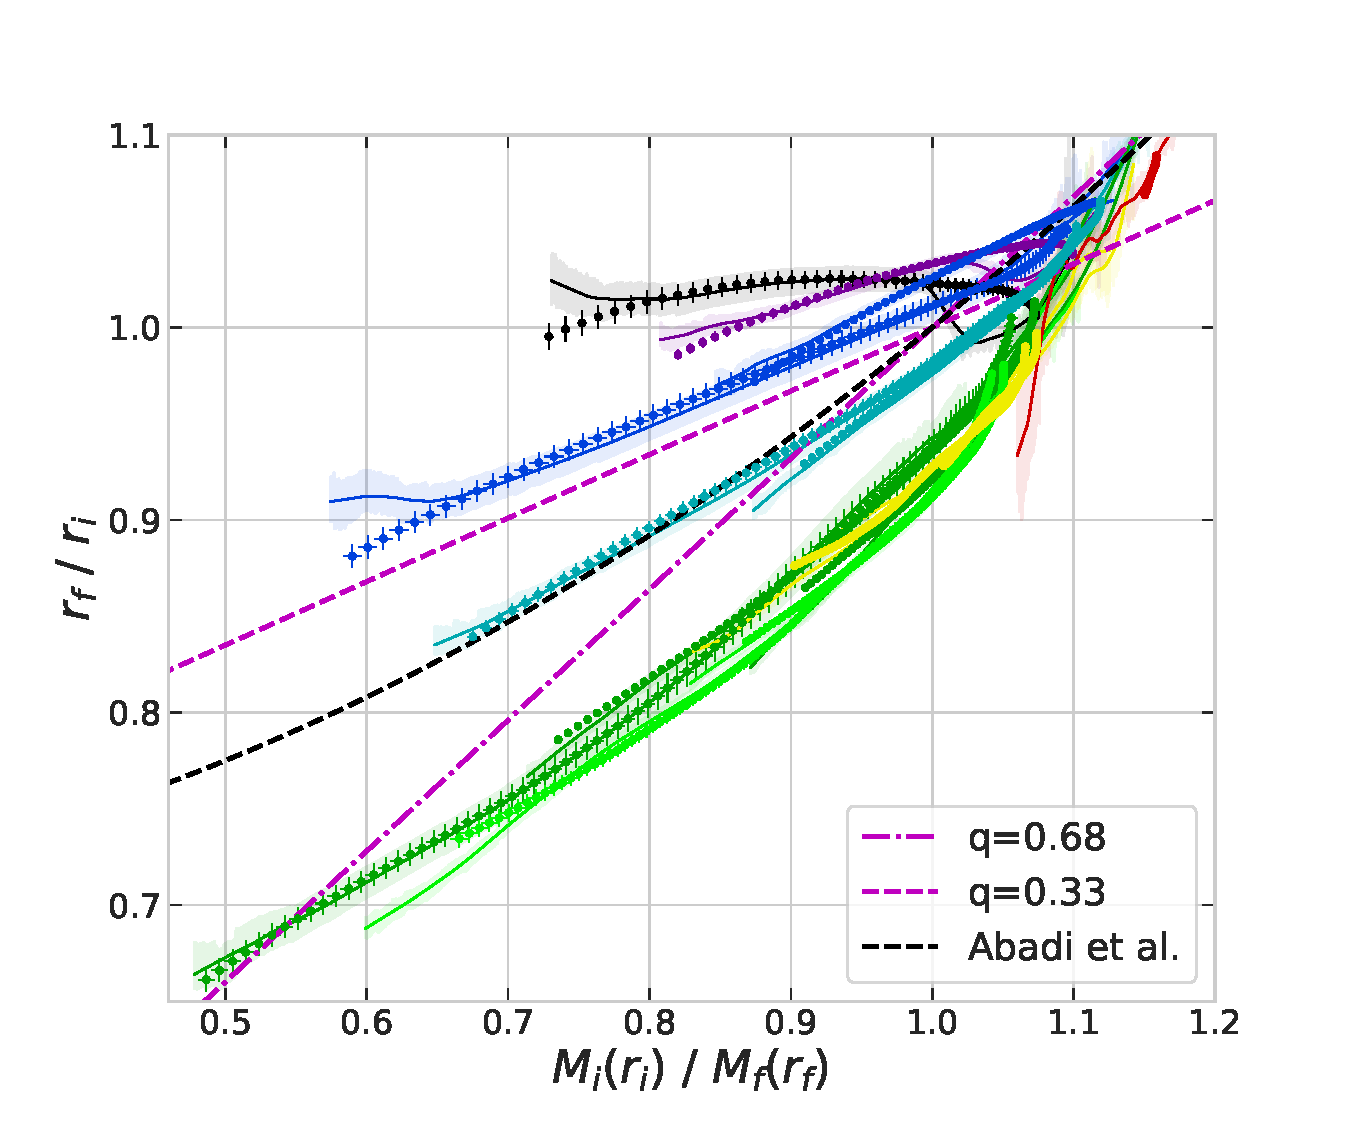
\includegraphics[width=0.48\linewidth]{plots/fit_view_M_T_snap098.pdf}
\caption{The stacked relation between relaxation ratio and mass ratio as a function of halo mass in IllustrisTNG at $z=0$ \emph{(bottom right panel)} and $z=1$ \emph{(other panels)}. In the top right panel, relaxation is shown at $z=1$ for the progenitors of the haloes selected at $z=0$. In the second row, left panel, relaxation is shown at different mass bins at $z=1$, indicated by corresponding mass bins at $z=0$. Points represent stacks over fixed halo-centric distances, and solid lines represent stacks over fixed mass ratios. The color-coding follows Fig.~\ref{fig:mass_bin_label-z01}. The quasi-adiabatic relaxation model \eqref{eq:chi-linear-ch:sims} with $q=0.68$ and $q=0.33$ are shown by the dot-dashed and dashed purple lines, respectively, in each panel.}
\label{fig:fit-view-mass-indep}
\end{figure*}

In \chapref{chap:z0_main}, we proposed a locally linear model of the relaxation relation as follows:
\begin{align}
\label{eq:chi-linear-q0-ch:physvar}
\frac{r_f}{r_i} - 1 &= q_1(r_f) \left[ \frac{M_i(r_i)}{M_f(r_f)} - 1 \right] + q_0(r_f),.
\end{align}
We have tested this relation with our halo samples at $z=1$ and found it to hold reasonably well. For each halo sample, at each $r_f$, the relationship between mass ratio and relaxation ratio across all haloes is fitted by a linear curve to obtain the parameters $q_0(r_f)$ and $q_1(r_f)$. These radial profiles of the relaxation parameters are shown in \figref{fig:rf-fit-params}.

The universality in these profiles extends to much larger mass haloes ($\sim 10^{13.5} \Mh$) at $z=1$ (top left panel) compared to $z=0$ (bottom right panel). This universality extends across all halo samples especially when considering all haloes identified by the median progenitor mass (shown in bottom left panel). Also we note that these radially-dependent relaxation results differ noticeably between bottom left panel and the top right panel. For example, in large clusters ($10^{14} \Mh$), the overall relaxation relation remains the same (black curves in \figref{fig:fit-view-mass-indep}), following the $q=0.33$ model. However, they differ when analyzed through the radially dependent relaxation model, as seen in \figref{fig:rf-fit-params} by comparing the black curves between the top right and bottom left panels.

The offset parameter $q_0$ shown in the lower subpanels is relatively uniform across the halo in all populations. The \figref{fig:fit-fit-func-q} shows the mean of $q_0$ in all four sets of halo samples. The $q_0$ parameter is usually more negative across all $z=1$ halo populations compared to $z=0$, indicating a stronger relaxation offset. Additionally, the values are more universal with halo mass at $z=1$. 


\begin{figure}[htbp]
\centering
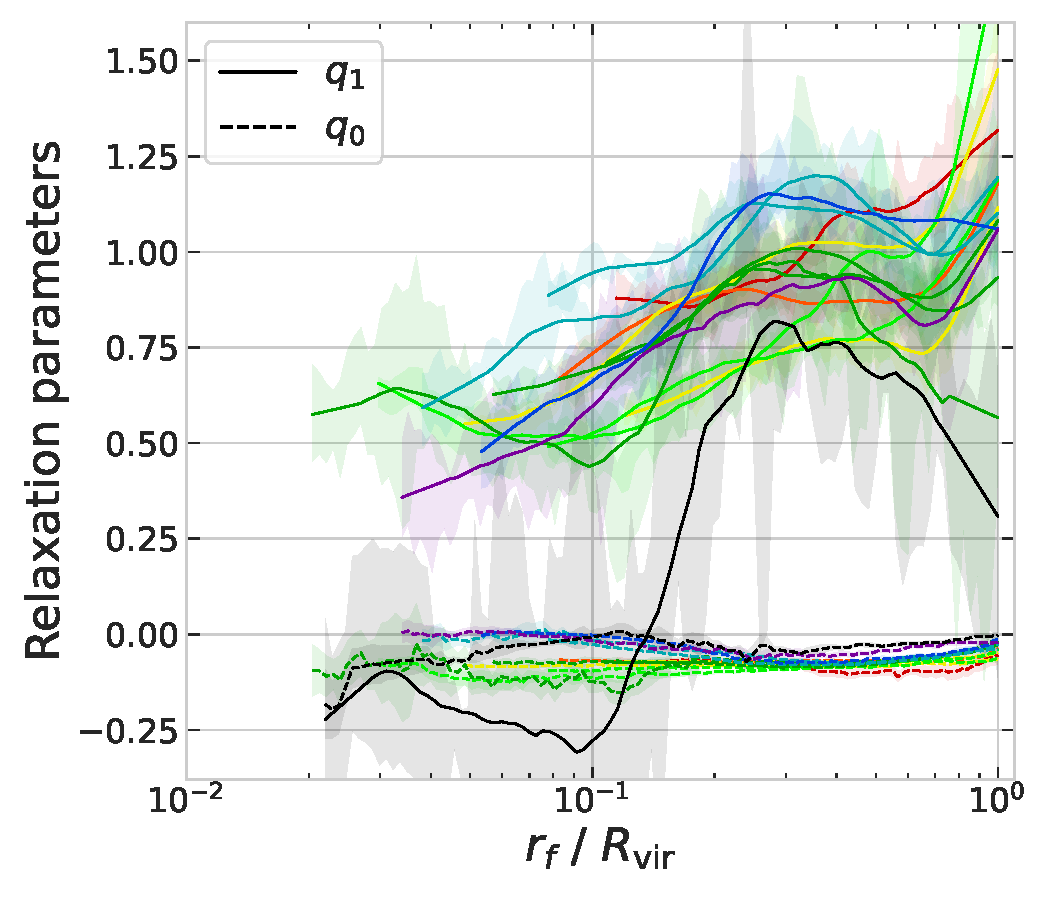
\includegraphics[width=0.48\linewidth,trim={0.5cm 0 0 0},clip]{plots/fit_params_rf_M_T_snap049.pdf}
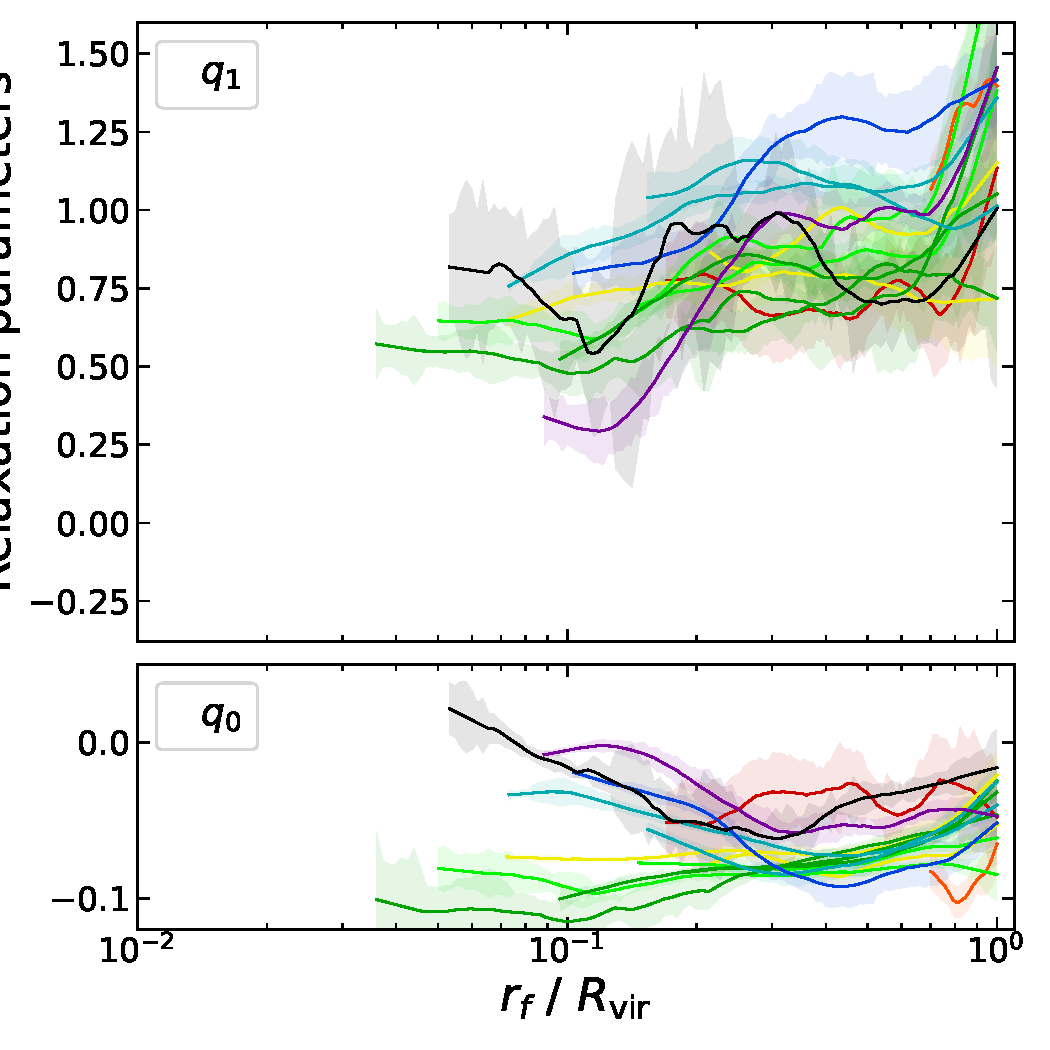
\includegraphics[width=0.48\linewidth,trim={0.5cm 0 0 0},clip]{plots/fit_params_rf_M_T_snap049_smpl98.pdf}
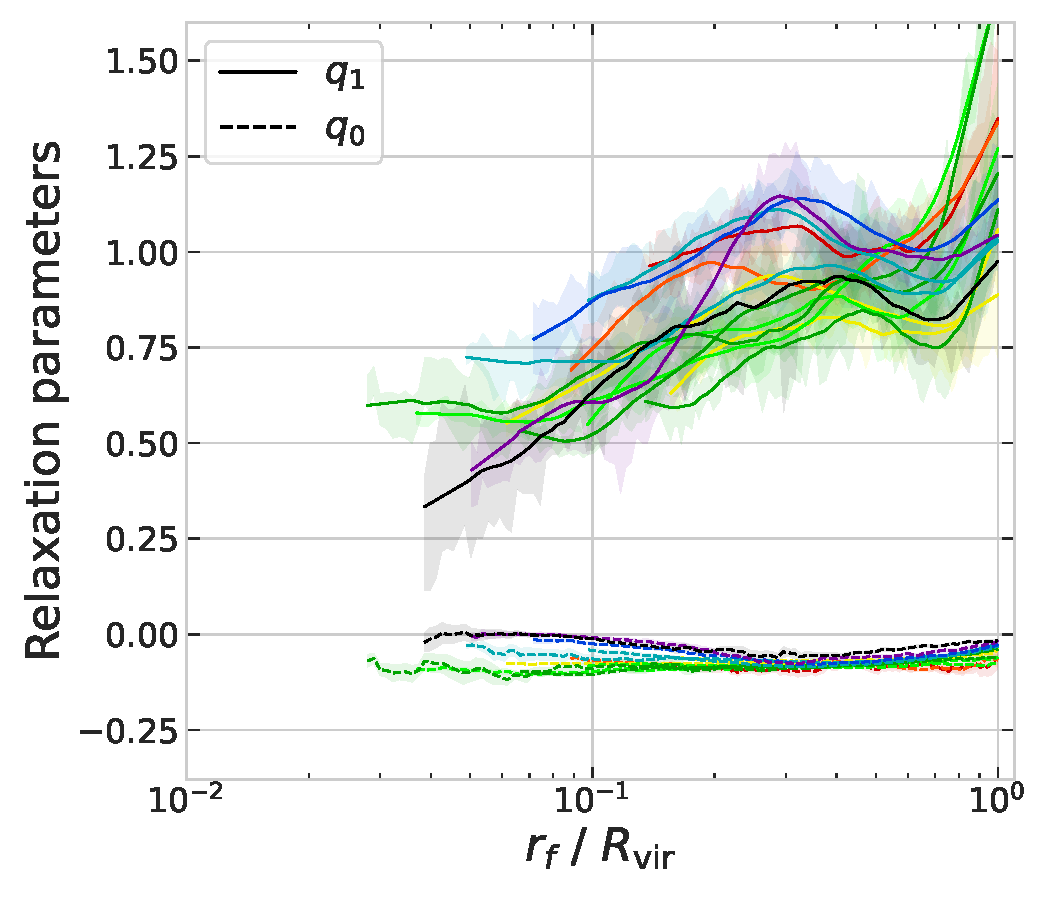
\includegraphics[width=0.48\linewidth,trim={0.5cm 0 0 0},clip]{plots/fit_params_rf_M_T_snap049_smpl98_allHalsMrange.pdf}
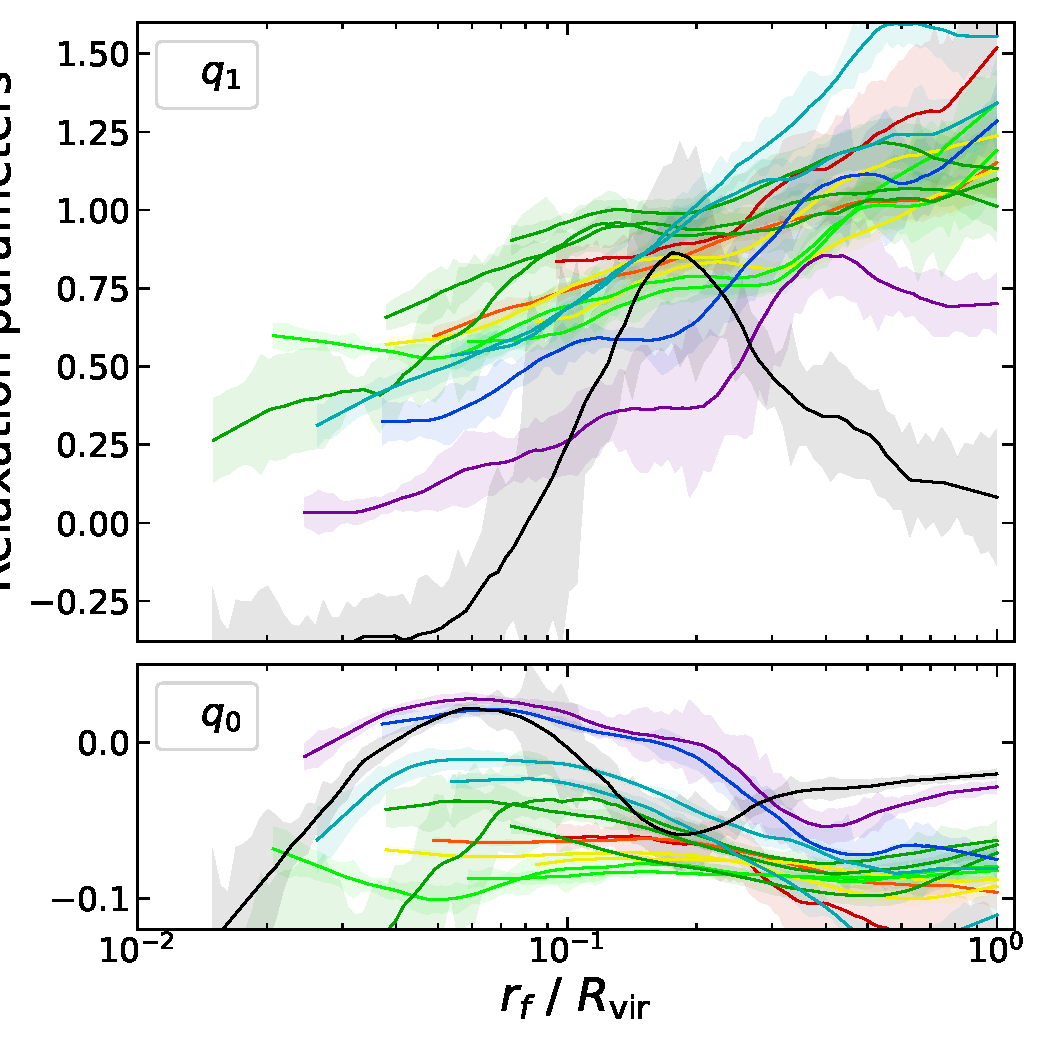
\includegraphics[width=0.48\linewidth,trim={0.5cm 0 0 0},clip]{plots/fit_params_rf_M_T_snap098.pdf}
\caption{Linear quasi-adiabatic relaxation model parameters $q_1$ and $q_0$ as a function of the halo-centric distance at different halo masses in IllustrisTNG at $z=0$ \emph{(bottom right panel)} and $z=1$ \emph{(other panels)}. In the top right panel, relaxation is shown at $z=1$ for the progenitors of the haloes selected at $z=0$. In the second row, left panel, relaxation is shown at different mass bins at $z=1$, indicated by corresponding mass bins at $z=0$. The color-coding follows Fig.~\ref{fig:mass_bin_label-z01}.}
\label{fig:rf-fit-params}
\end{figure}

\begin{figure}[htbp]
\centering
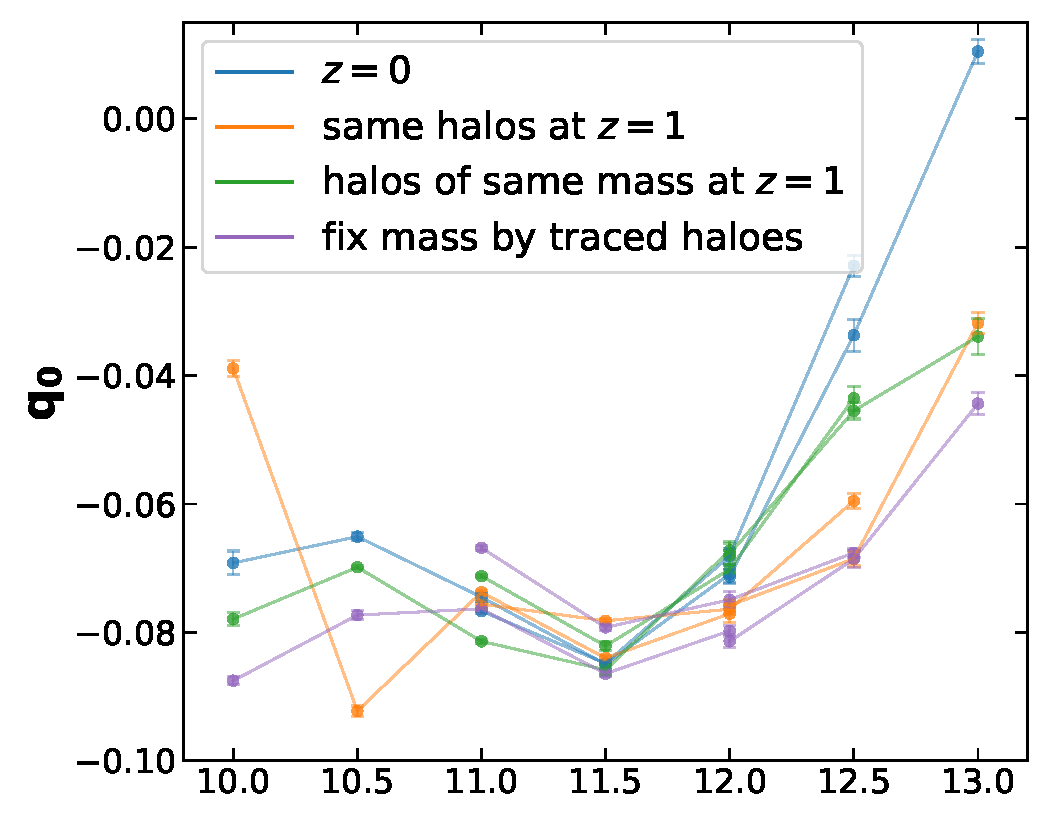
\includegraphics[width=0.6\linewidth]{plots/fit_param_q0_M_T_z01.pdf}
\caption{Mean of the radially dependent quasi-adiabatic relaxation offset, $q_{0}$ as a function halo mass in the four sets of halo samples indicated by color.}
\label{fig:fit-fit-func-q}
\end{figure}










\section{Variation in astrophysical feedback using CAMELS simulations}
\label{sec:res-physvar-CAMELS}
In this section, we present the role of various feedback parameters prescribed in the IllustrisTNG simulations using set of CAMELS simulations performed with the IllustrisTNG model. This includes a set of 41 hydrodynamical simulations, with one replicating the reference TNG model in the smaller cosmological volume, and 10 simulations each by varying 4 different feedback parameters as described in \secref{sec:sims-CAMELS}. To recall, this includes two supernovae feedback parameters ($A_{\mathrm{SN1}}$ and $A_{\mathrm{SN2}}$) and another two AGN feedback parameters ($A_{\mathrm{AGN1}}$ and $A_{\mathrm{AGN2}}$). 

% Let us first focus on the relaxation characterised by the intercepts in the relaxation relation of individual haloes. 

% \subsubsection*{Model independent relaxation offset}

Due to the limited resolution and the smaller volumes of the CAMELS simulation, among all the mass bins shown in \figref{fig:mass_bin_label-z01}, we consider only $10^{11} \Mh$, $10^{11.5}$ and $10^{12} \Mh$ at both redshifts $z=0$ and $z=1$. Even in these mass bins we consider only the outer well resolved regions of the haloes. Also since the cosmological volume is smaller than even the smallest TNG50 simulation, we have only smaller sample of haloes at each of this halo mass bins. We find this sample size insufficient to estimate the radially-dependent relaxation parameters at each of this mass bin. We consider the following two approaches to alleviate this issue. 

\subsection*{Intercepts in the Relaxation Relaxation}

The intercepts of the relaxation relation, given by the relation between $M_i/M_f-1$ and $r_f/r_i-1$ already give interesting information about the relaxation.
For example, the y-intercept denotes the offset in the relaxation ratio $rf/ri$ from unity for the shells having a mass ratio of unity $M_i/M_f=1$. And similarly the x-intercept denotes the offset in the mass ratio $M_i/M_f$ from unity for the shells having a relaxation ratio $rf/ri = 1$ of unity.

In a given sample of haloes, we denote the average x and y intercepts as $q_x$ and $q_y$ respectively. For example, if we consider the Milky Way scale haloes at redshift $z=0$, the relaxation relation shown by the green curves in lower right panel of \figref{fig:fit-view-mass-indep} indicate that the $q_x$ will be positive and $q_y$ will be negative. In general, we expect that feedback effects would lead to larger $q_x$ and more negative $q_y$.

Due to the limited resolution of the CAMELS simulation, the outer well-resolved regions in most of haloes didn't had a mass ratio less than unity. This makes the y-intercept of the relaxation relation available only in smaller number of haloes. This makes our estimation of $q_y$, very noisy and hence we only interpret the parameter $q_x$ in these simulations. This parameter $q_x$ is presented in the \figref{fig:camels-qx0} as a function of the astrophysical parameters in the CAMELS TNG set of simulations at both redshifts $z=0$ and $z=1$.

\subsection*{Wider mass bin}
We found that the radially-dependent relaxation parameters are usually more uniform across a wider range of halo masses. We leverage this to consider haloes in a wider mass bin from $10^{11}\Mh$ to $10^{12}\Mh$, this gives a sufficient number of haloes to obtain the radially-dependent relaxation model parameters.
However still, the radial range is not sufficient to accurately model the radial dependence of the slope parameter $q_1(r_f)$, we only investigate the offset parameter $q_0$ defined as the mean of the $q_0(r_f)$. This parameter $q_0$ is usually negative and it is expected to be more negative when offset produced by overall feedback effects are stronger. This model-dependent offset parameter is present in \figref{fig:camels-q0q1} at both redshifts $z=0$ and $z=1$.

\subsection*{Discussion}
We find that among all haloes investigated, the feedback strength parameters $A_{\mathrm{SN1}}$ and $A_{\mathrm{AGN1}}$ have a strong influence on the relaxation, however, the wind speed parameters $A_{\mathrm{SN2}}$ and $A_{\mathrm{AGN2}}$ have negligible effect on the relaxation characterized by $q_x$ and $q_0$. 

Recall that when varying only a wind speed parameter it affects the burstiness of the feedback outflows keeping the overall flux constant. Suppose the deviations in the relaxation relation from idealized adiabatic model, quantified by non-zero these offset parameters is caused by the transfer of angular momentum between the dark matter particles and the baryonic particle. Then one may expect that the nature of the baryonic feedback quantified by the wind speed parameters will have significant influence on the value of $q_x$; Our results suggest otherwise. 

This suggests that the strong influence of the overall feedback outflow flux on the relaxation is likely due to the time delay in the relaxation response of the halo. Also, the larger offsets characterized by $q_x$ in \figref{fig:camels-qx0},with stronger feedback implementation is consistent with our discussion in \secref{subsubsec:sim-relax-ch:z0main}. 

We find that the AGN feedback strength has generally stronger influence on the relaxation among the high mass haloes, whereas the supernova feedback strength have stronger influence in lower mass haloes. This is consistent with our expectations that the AGN feedbacks dominate in more massive haloes. However, at all masses AGN feedbacks starts dominating the value of $q_x$ with unrealistically strong AGN feedback implementations, this is indicated by the green curves in \figref{fig:camels-qx0}. 

The relaxation offset in the outer region of haloes characterised by $q_x$ is always larger with the stronger implementation of AGN feedback at both \( z=0 \) and \( z=1 \). However, in the slightly inner regions, stronger AGN feedback implementation leads to a weaker relaxation offset at \( z=0 \) and a stronger offset at \( z=1 \). We interpret this as a consequence of the overall reduction in total feedback at \( z=0 \) due to the suppression of star formation caused by higher AGN feedbacks in the past. These results highlight the significance of feedback mechanisms in building a physical understanding of dark matter halo relaxation.

We find that at $z=1$, the magnitude of $q_0$ is larger with stronger AGN feedback indicated by larger $A_{\rm{AGN1}}$. However this trend is absent is totally absent in $z=0$. This could be because of a strong suppression in star formation rate at present epoch due to the stronger AGN feedback in the past.
\begin{figure}[htbp]
\centering
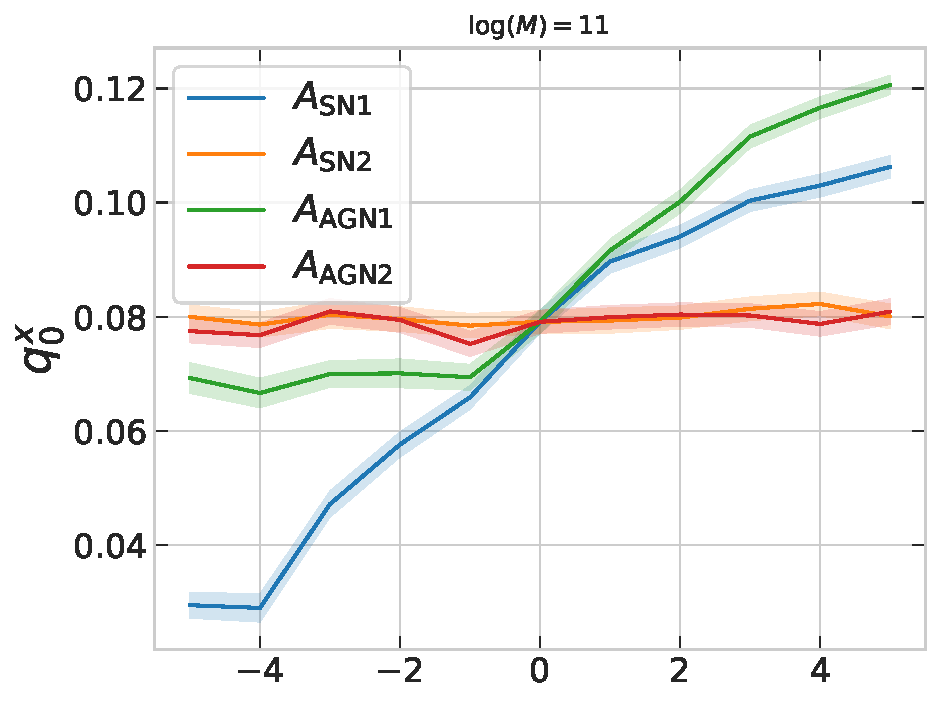
\includegraphics[width=0.325\linewidth]{plots/CAMELS_I_qx0_sn18_11.pdf}
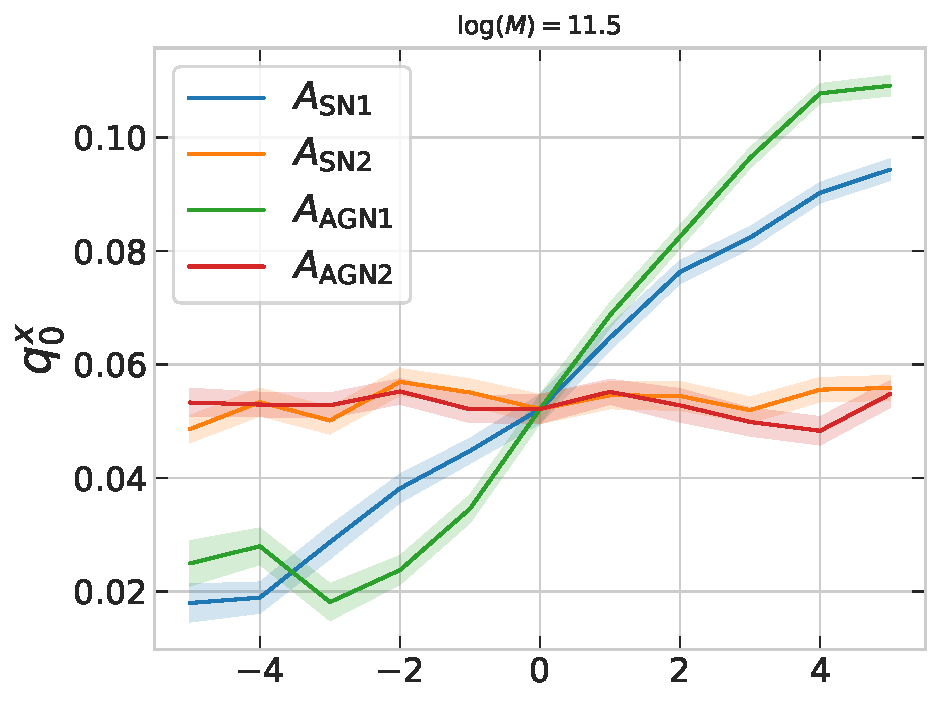
\includegraphics[width=0.325\linewidth]{plots/CAMELS_I_qx0_sn18_11.5.pdf}
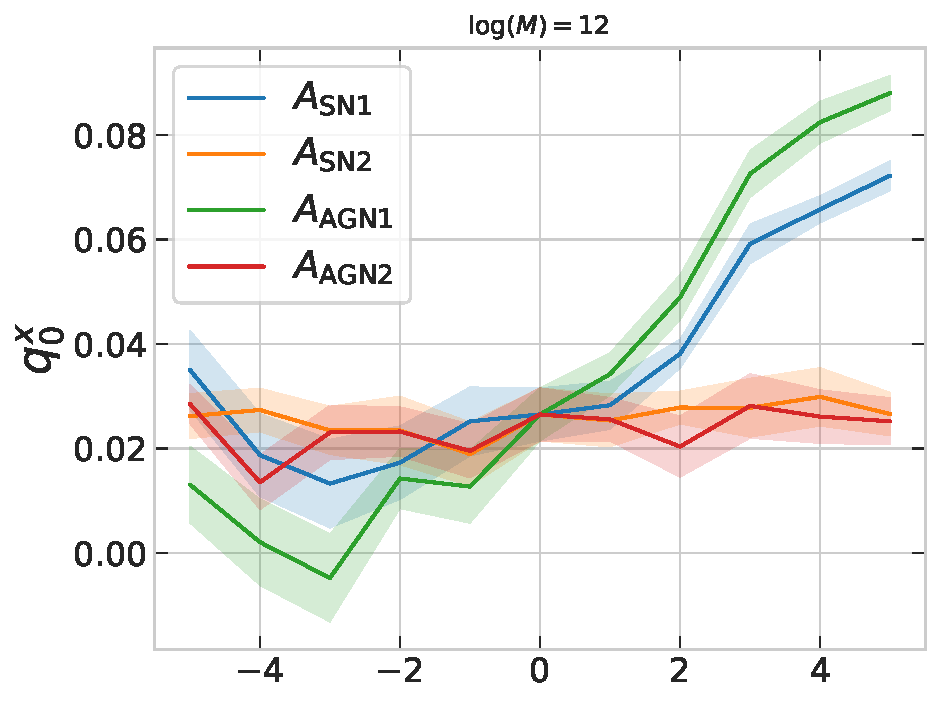
\includegraphics[width=0.325\linewidth]{plots/CAMELS_I_qx0_sn18_12.pdf}
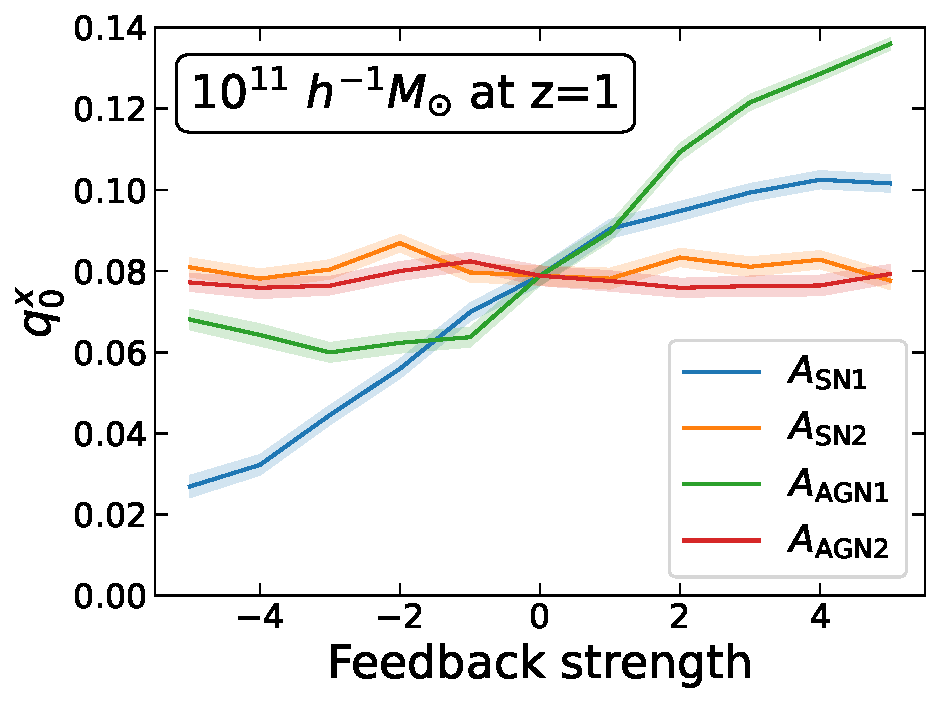
\includegraphics[width=0.325\linewidth]{plots/CAMELS_I_qx0_sn33_11.pdf}
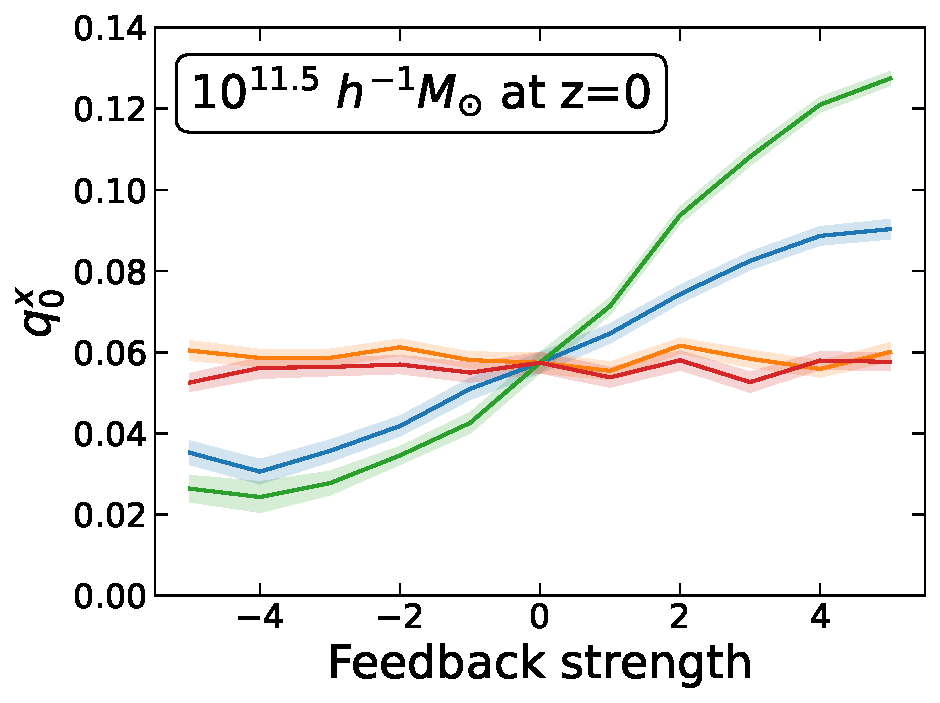
\includegraphics[width=0.325\linewidth]{plots/CAMELS_I_qx0_sn33_11.5.pdf}
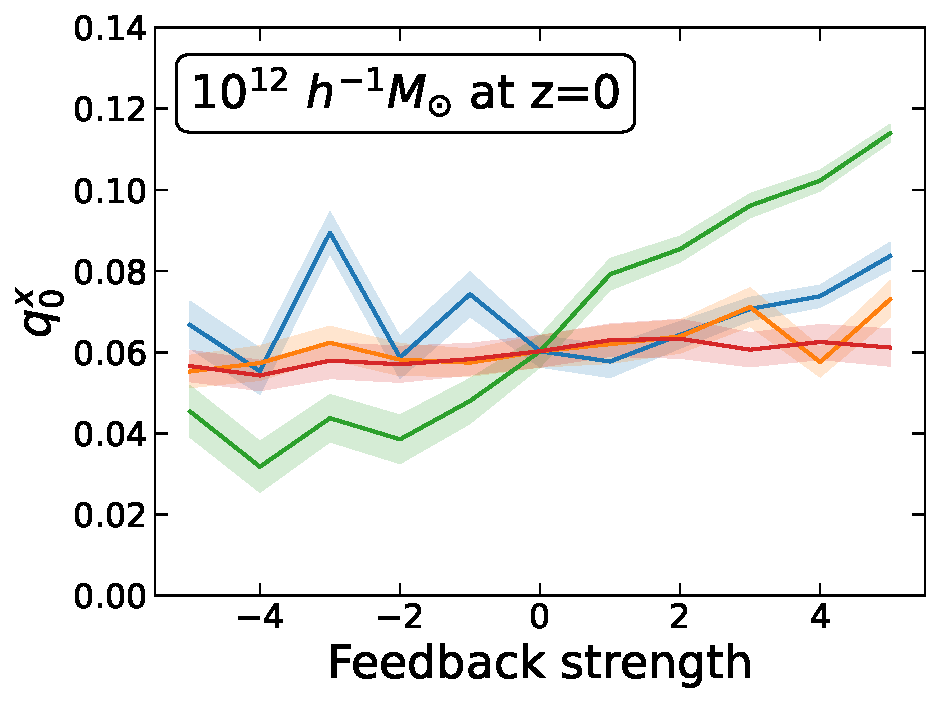
\includegraphics[width=0.325\linewidth]{plots/CAMELS_I_qx0_sn33_12.pdf}
\caption[]{Relaxation offset parameter $q_x$ as a function of the baryonic astrophysical feedback parameters in haloes found in CAMELS-TNG at three different halo masses. Top: z=1, Bottom: z=0}
\label{fig:camels-qx0}
\end{figure}




% \begin{figure}[htbp]
% \centering
% 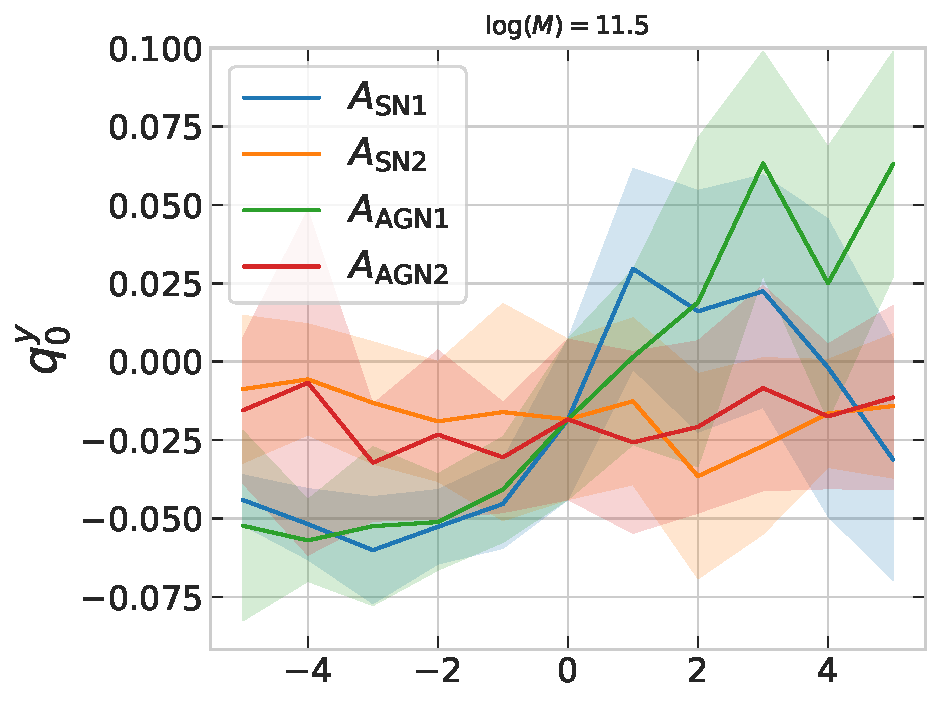
\includegraphics[width=0.325\linewidth]{plots/CAMELS_I_qy0_sn18_11.5.pdf}
% 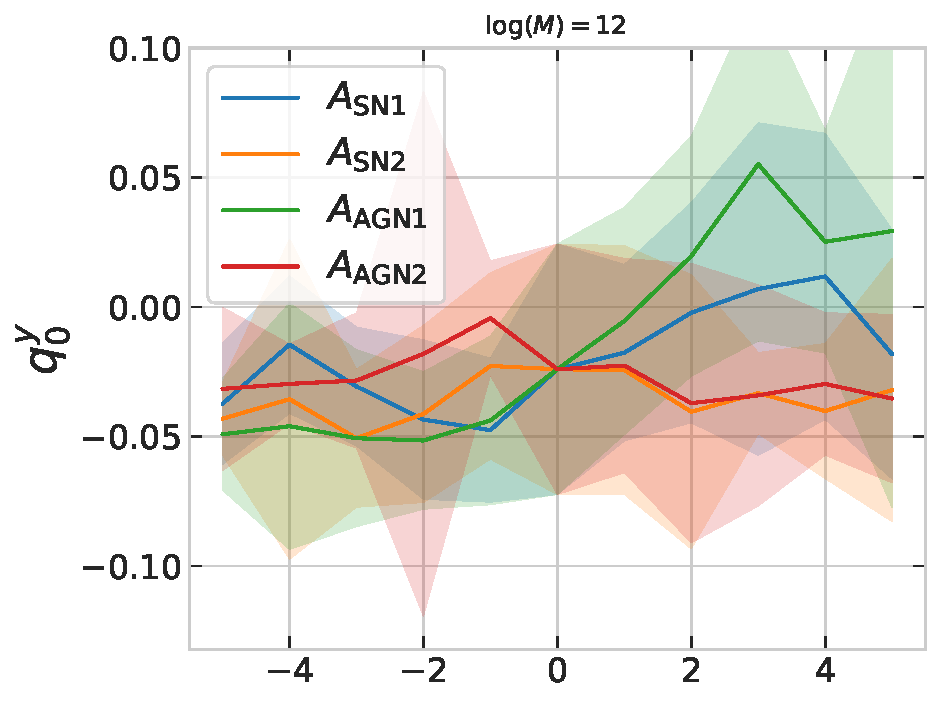
\includegraphics[width=0.325\linewidth]{plots/CAMELS_I_qy0_sn18_12.pdf}
% 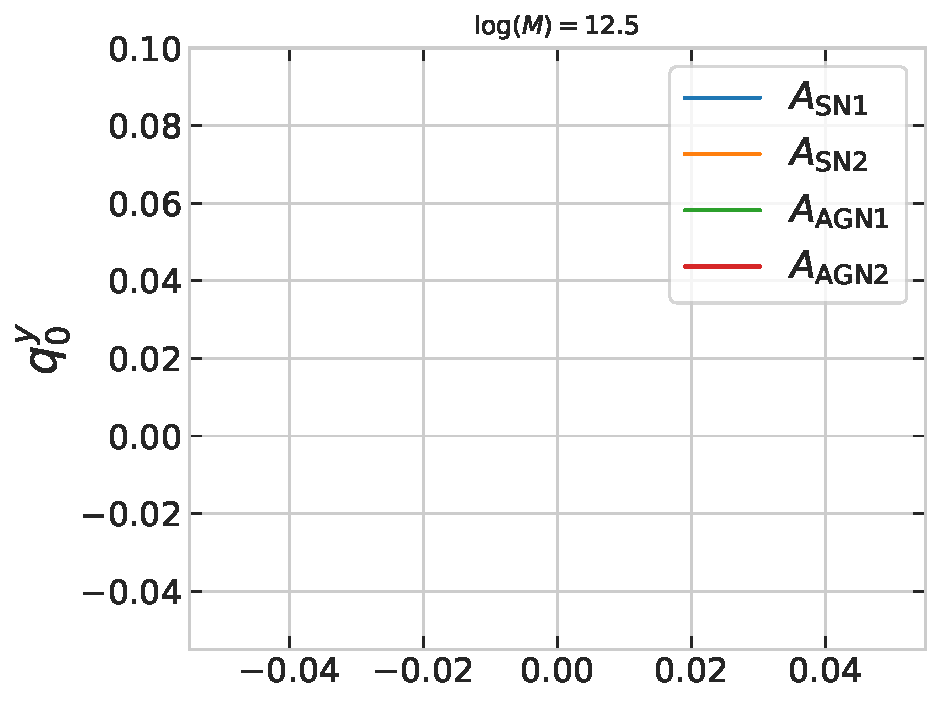
\includegraphics[width=0.325\linewidth]{plots/CAMELS_I_qy0_sn18_12.5.pdf}
% 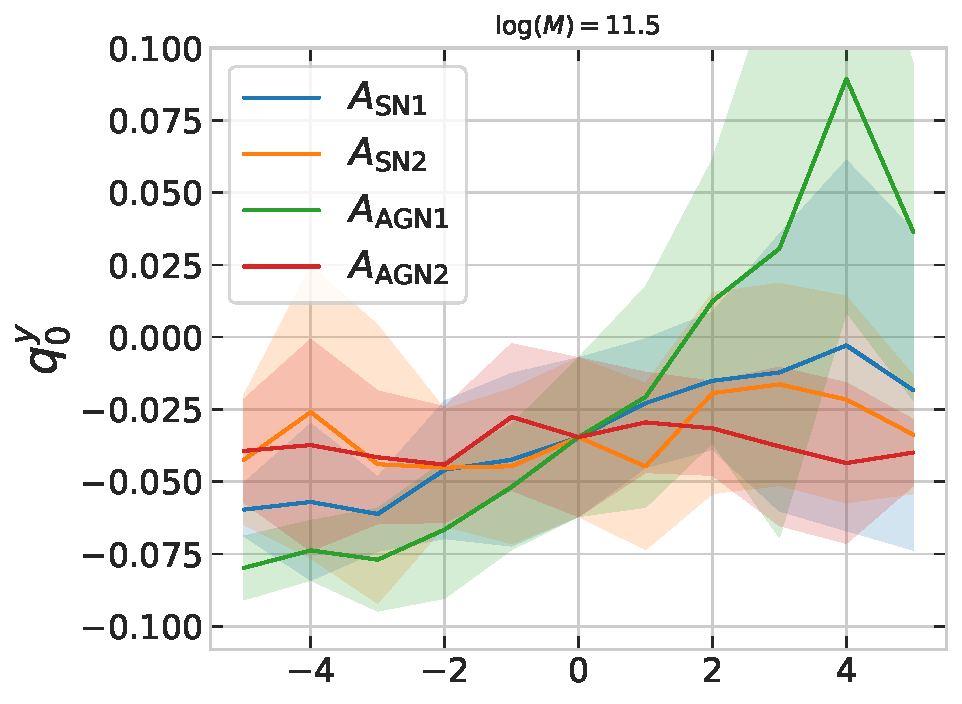
\includegraphics[width=0.325\linewidth]{plots/CAMELS_I_qy0_sn33_11.5.pdf}
% 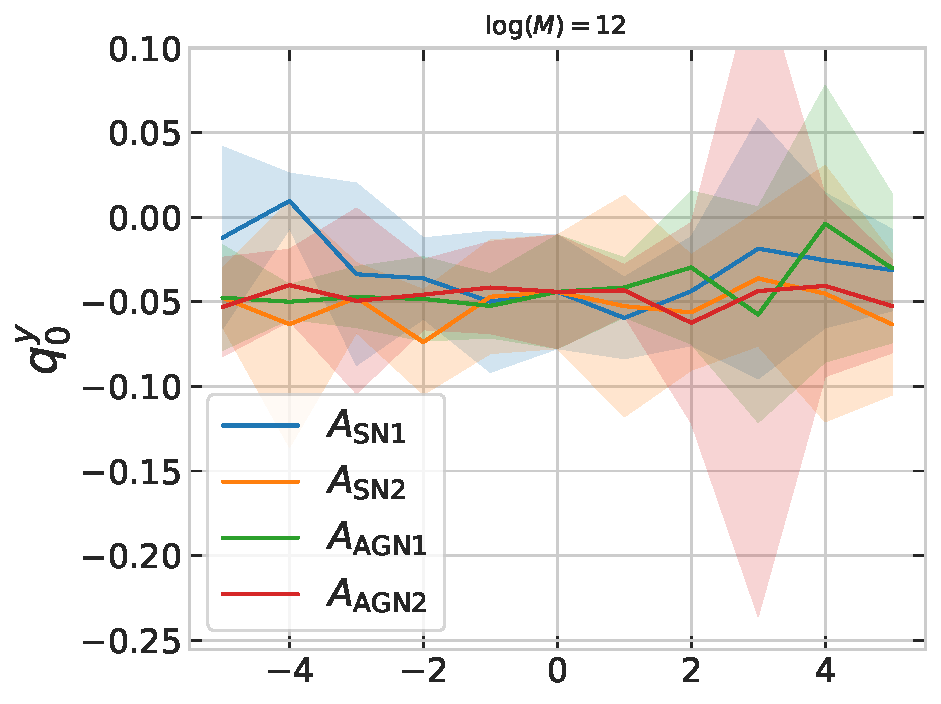
\includegraphics[width=0.325\linewidth]{plots/CAMELS_I_qy0_sn33_12.pdf}
% 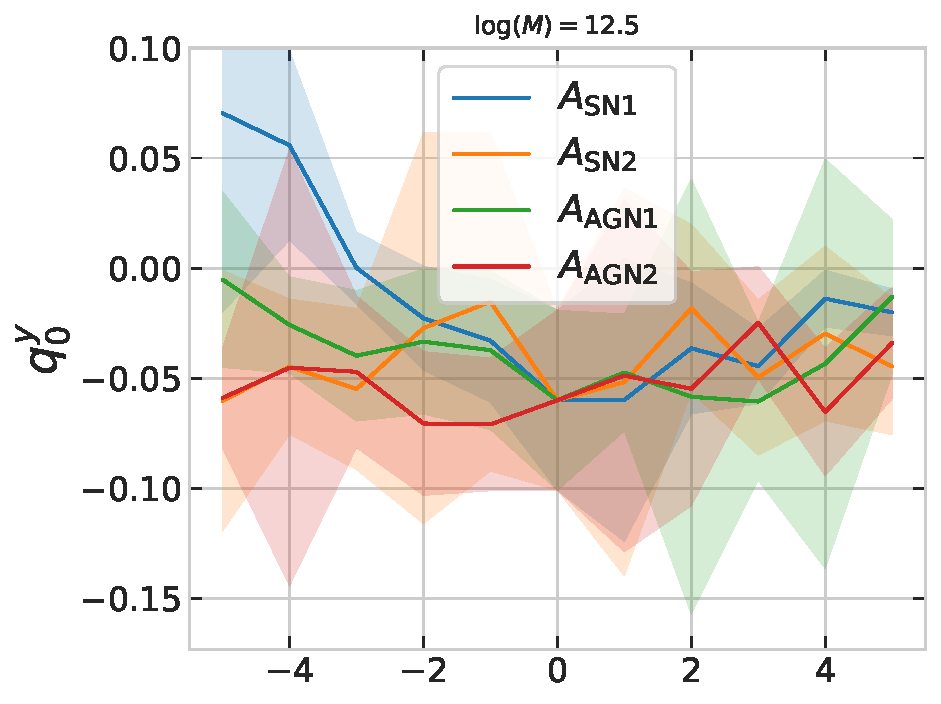
\includegraphics[width=0.325\linewidth]{plots/CAMELS_I_qy0_sn33_12.5.pdf}
% \caption[]{Response as a function of baryonic parameters in CAMELS-TNG. \\\hspace{\textwidth}Top: $z=1$, Bottom: $z=0$.}
% \label{fig:camels-qy0}
% \end{figure}
\begin{figure}[htbp]
\centering
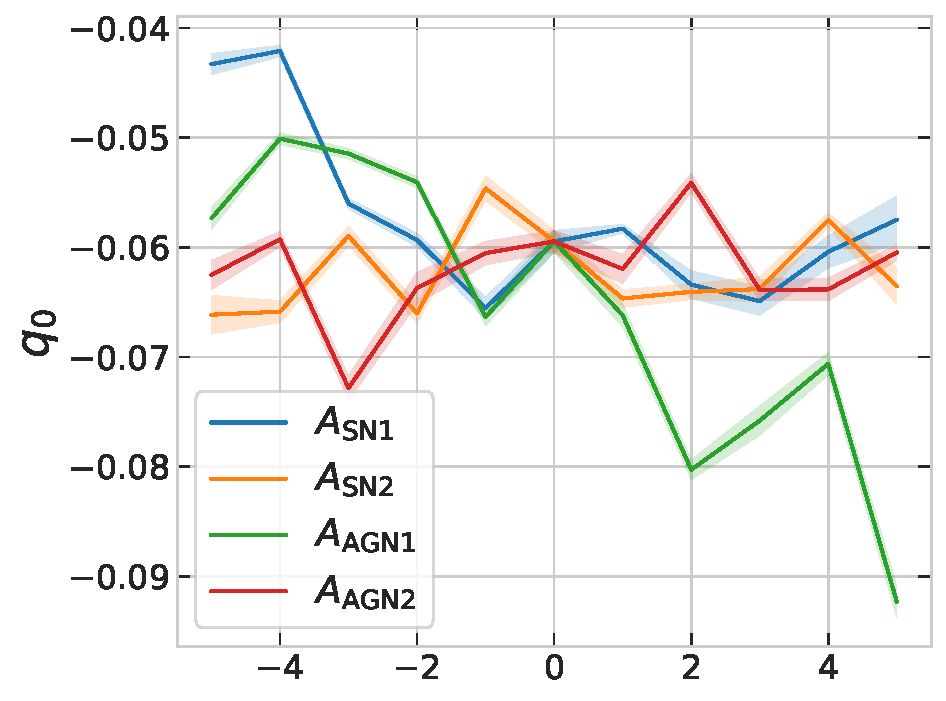
\includegraphics[width=0.49\linewidth]{plots/CAMELS_I_q0_sn18.pdf}
% 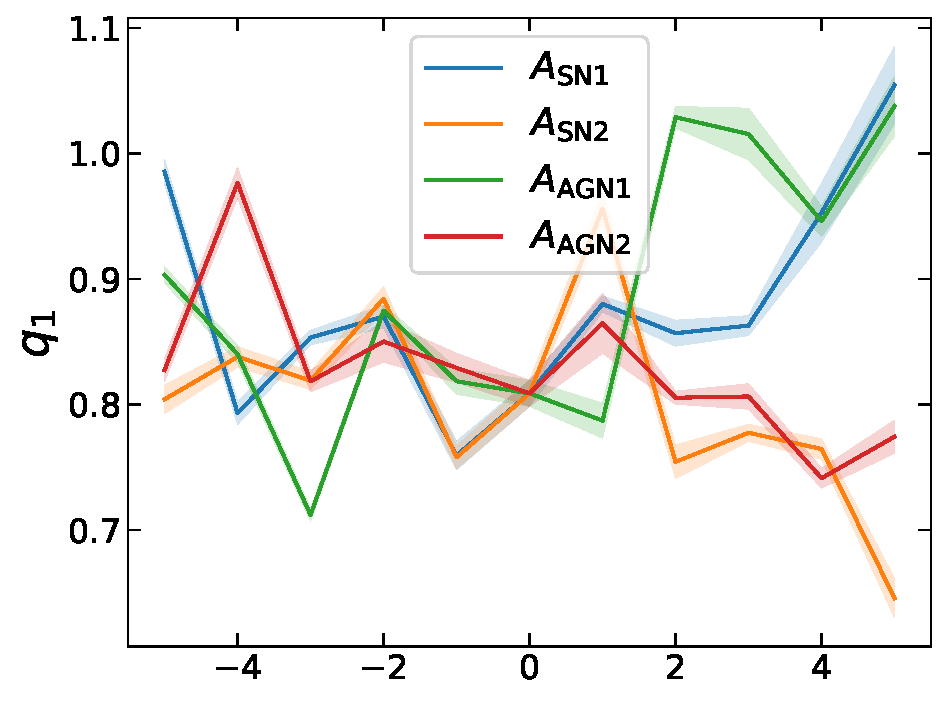
\includegraphics[width=0.49\linewidth]{plots/CAMELS_I_q1_sn18.pdf}
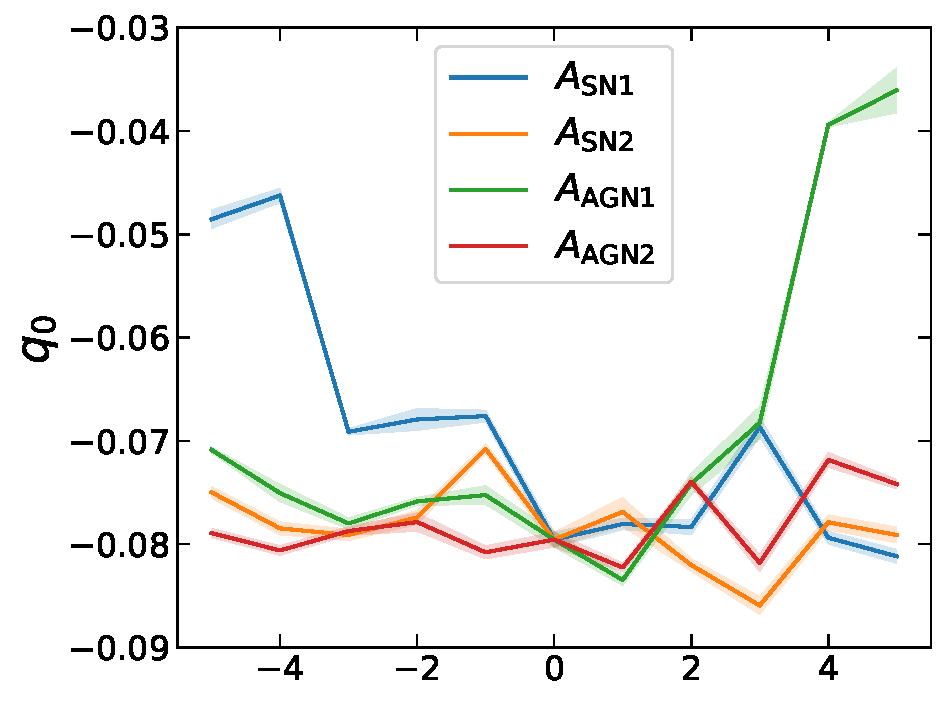
\includegraphics[width=0.49\linewidth]{plots/CAMELS_I_q0_sn33.pdf}
% 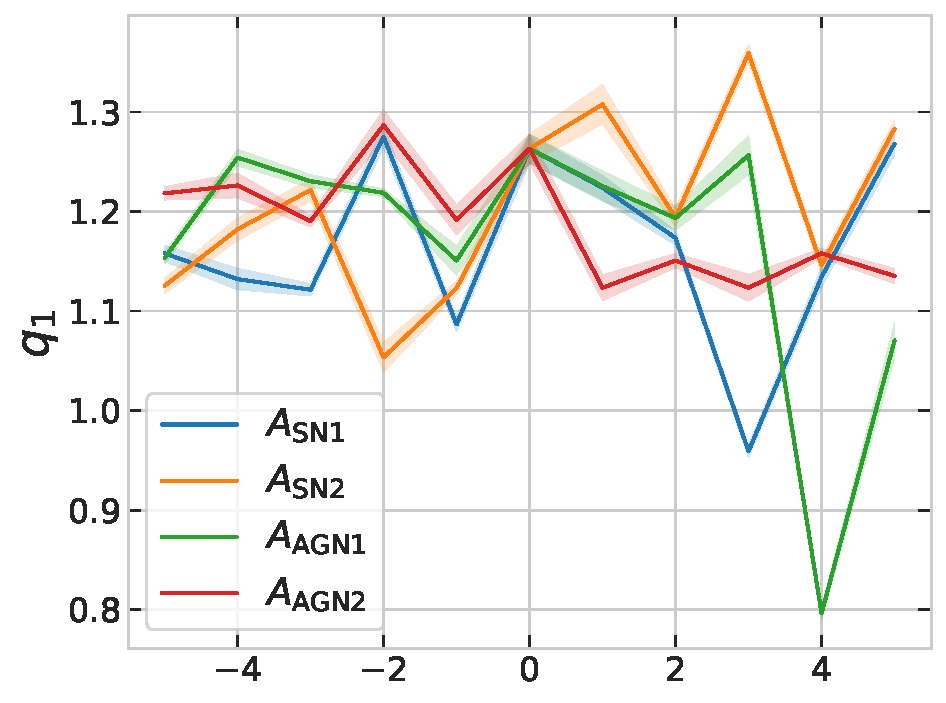
\includegraphics[width=0.49\linewidth]{plots/CAMELS_I_q1_sn33.pdf}
\caption[]{Relaxation offset parameter $q_0$ as a function of the baryonic feedback parameters in CAMELS-TNG. Left: $z=1$, Right: $z=0$.}
\label{fig:camels-q0q1}
\end{figure}









\section{Role of astrophysical models in EAGLE simulations}
\label{sec:res-physvar-eagle}
In this section, we present insights from small boxes of EAGLE simulations on the role of different feedback mechanisms on the relaxation response. These physics variation simulations from the EAGLE suite are described in \secref{sec:sims-EAGLE}. Again due to the significantly smaller box size and the resolution, we only consider haloes in three different mass bins centred at $10^{10.5 \Mh}$, $10^{11} \Mh$ and $10^{11.5} \Mh$ as discussed in \secref{sec:res-physvar-CAMELS}. In these narrow mass bins, the mean relaxation relation obtained by stacking independent of the halo-centric distance is shown in \figref{fig:EAGLE-rad-indep} for these physics variation simulations. We find that the deviation in the relaxation across different astrophysical modelling is usually much smaller than the differences from one halo mass to the other. However, notice that the gas equation of state has a strong influence on the relaxation relation especially among low mass haloes. In particular, stiffer equations of state leads to a very large $r_f/r_i$ indicating a stronger expansion of the dark matter shells in response to galaxy formation.

In \figref{fig:EAGLE-rad-dep}, we present the radially dependent relaxation parameters for a larger sample haloes in wider range of halo masses from $10^{10.5 \Mh}$ to $10^{11.5} \Mh$. These result also reflect the strong influence of the equation of state of gas on the relaxation response of dark matter haloes. Additionally, these results highlight the effect of supernovae feedback modeling. In particular, the $q_0(r_f)$ is more negative indicating stronger offset in the haloes found in the simulation with stronger supernovae feedback implementation(brown curve vs rose curve).    

\begin{figure}[htbp]
\centering
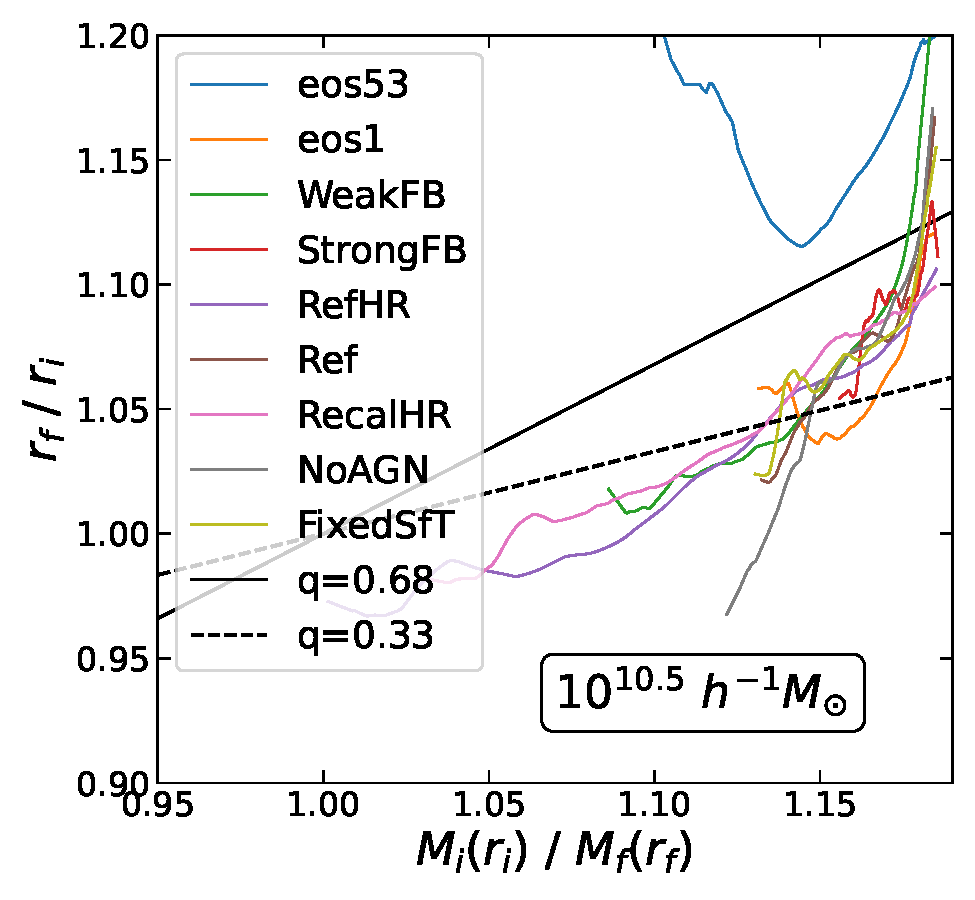
\includegraphics[width=0.32\linewidth]{plots/eagle_physvar_rad_indep_relxn_reln_MiMf_10.5.pdf}
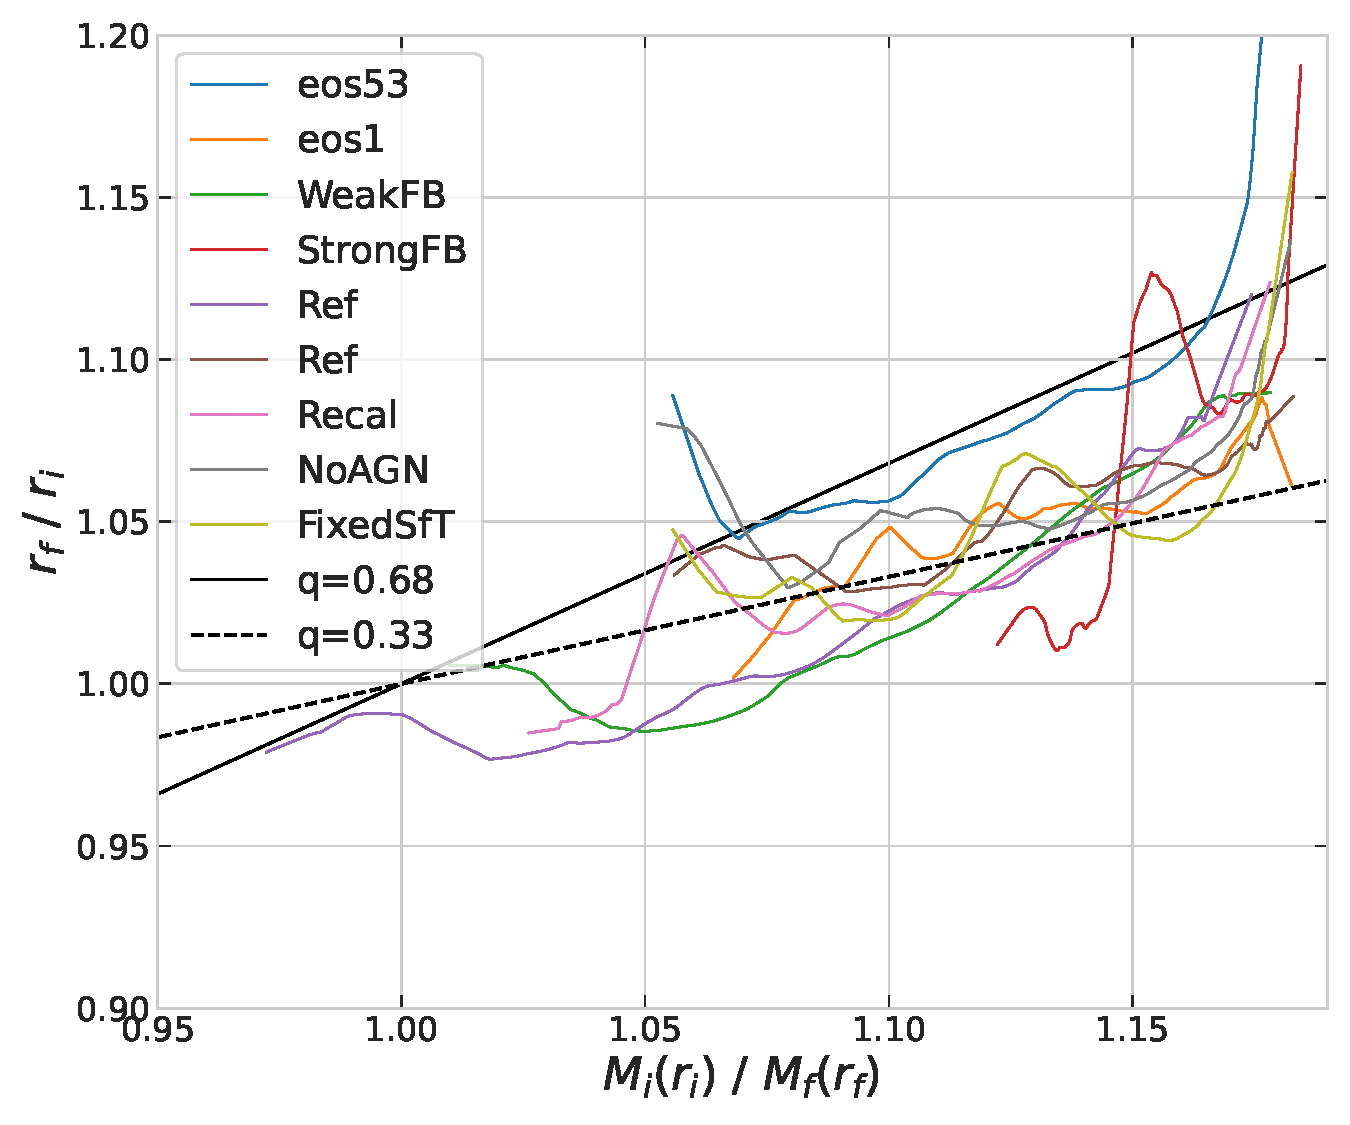
\includegraphics[width=0.32\linewidth]{plots/eagle_physvar_rad_indep_relxn_reln_MiMf_11.pdf}
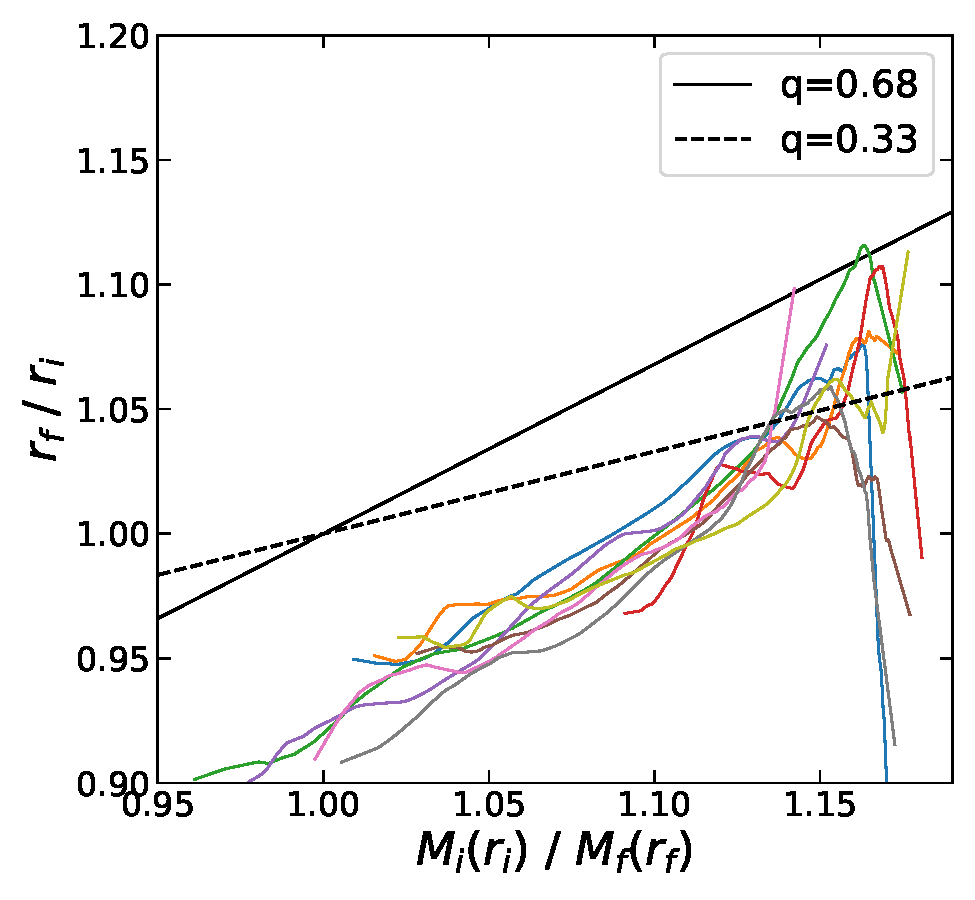
\includegraphics[width=0.32\linewidth]{plots/eagle_physvar_rad_indep_relxn_reln_MiMf_11.5.pdf}
\caption[]{Relaxation relation in the physics variation EAGLE simulations for haloes in the mass bins from $10^{10.5} \Mh$ to $10^{11.5} \Mh$.. Here colors represent the specific simulation with a variation in the baryonic physics prescription. } 
\label{fig:EAGLE-rad-indep}
\end{figure}

\begin{figure}[htbp]
\centering
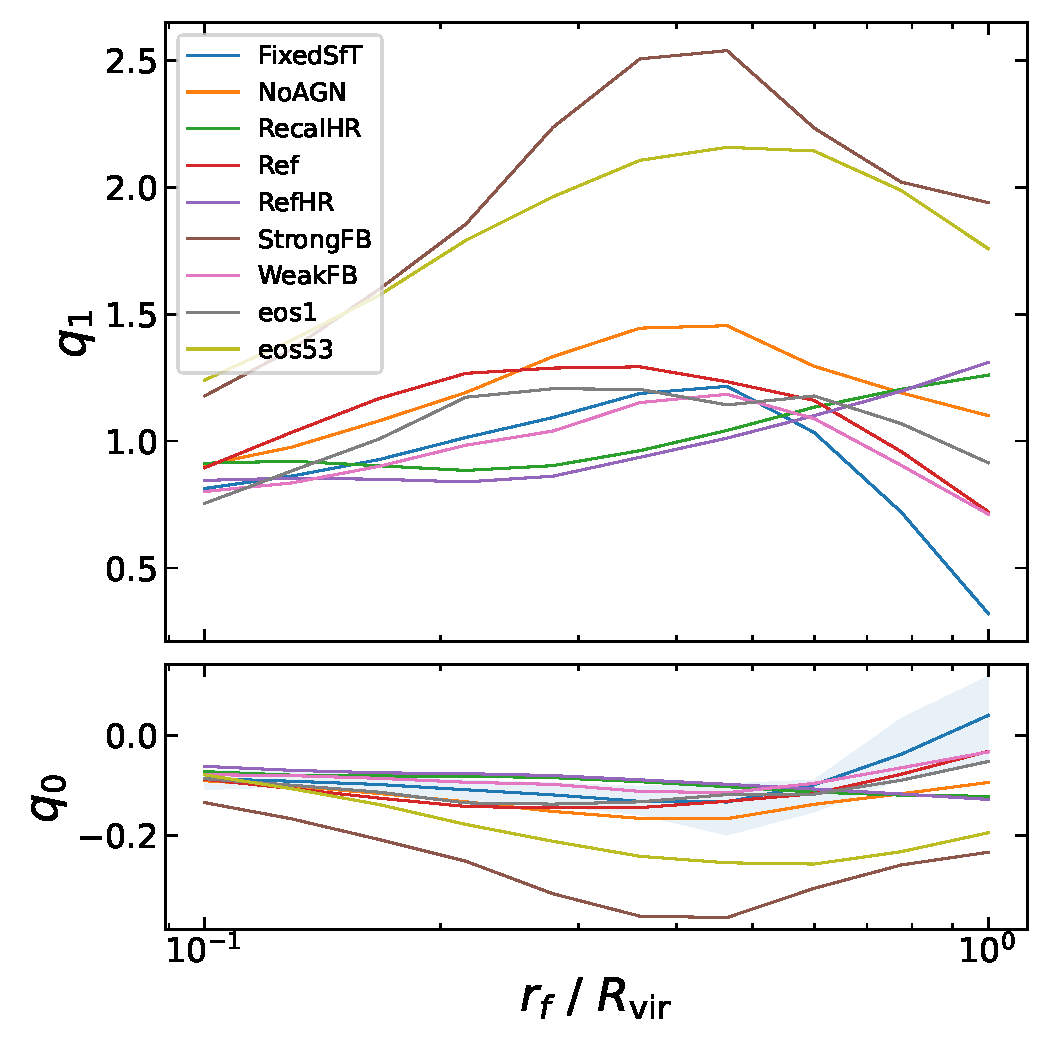
\includegraphics[width=0.7\linewidth]{plots/fit_params_rf_M_E_physvar_fatmass_uniradb.pdf}
\caption[]{Radially-dependent relaxation parameters for low-mass haloes from $10^{10.5} \Mh$ to $10^{11.5} \Mh$ as a function of the halo-centric distance in the physics variation EAGLE simulations. Here colors represent the specific simulation with a variation in the baryonic physics prescription.}
\label{fig:EAGLE-rad-dep}
\end{figure}


\section{Conclusion}
\label{sec:conclusion-ch:physvar}

In this chapter, We investigated the influence of astrophysical modeling on the relaxation response of dark matter haloes at different epochs, specifically focusing on \( z=0 \) and \( z=1 \). The analysis is divided into three main parts, each shedding light on the role of various astrophysical processes in shaping the dark matter content of haloes.

% \subsubsection*{1. Early Epoch in IllustrisTNG Simulations}
We began by examining the relaxation response at an earlier redshift (\( z=1 \)) in the IllustrisTNG simulations using three distinct set of halo samples, which highlight the variations in relaxation across different halo masses. Our study reveals that dark matter relaxation tends to be usually stronger (smaller \(r_f/r_i\)) at the earlier epoch compared to the present among haloes of the same mass. This is even more prominent among the progenitors of present epoch haloes. Notably, we observe that cluster-scale haloes at \( z=1 \) show significant relaxation (\(r_f/r_i<1\)) that is also a function of the change in the enclosed mass (\(M_i/M_f\)). This is in contrast to similar haloes at the present epoch, where \(r_f/r_i\) stayed close to unity on average irrespective of the value of \(M_i/M_f\).

We also find that the locally linear quasi-adiabatic relaxation model is also a good description of the relaxation relation at this earlier epoch, demonstrating its robustness in capturing the dark matter response across redshifts. Moreover, the parameters of the radially dependent relaxation are found to be more universal across a much wider range of masses at \( z=1 \). For example, the progenitors of even the most massive clusters are well characterized by the simple three-parameter model of relaxation that was developed with a focus on galactic-scale haloes at \( z=0 \).

% \subsubsection*{2. Variation in Astrophysical Feedback Using CAMELS Simulations}
Next, we explore variations in astrophysical feedback strengths within the IllustrisTNG model using simulations from the CAMELS project, which varies four different feedback parameters: two for stellar feedback and two for AGN feedback. Our analysis shows that the parameters controlling the energy flux of the feedback have a significant impact on the relaxation of dark matter at different epochs. In contrast, the parameters governing the speed and burstiness of feedback have negligible effects on the halo relaxation response.

We find that variations in stellar feedback strengths have a larger impact among dwarf galaxy-scale haloes, while variations in AGN feedback parameters exert a stronger influence on Milky Way-scale haloes. Notably, the relaxation offset in the outer well-resolved regions is stronger at the present epoch than at \( z=1 \), contrasting with results from the inner regions explored in the IllustrisTNG simulations in the first part of this chapter.

The stronger implementation of AGN feedback tends to result in greater relaxation at both \( z=0 \) and \( z=1 \) in the outer regions of the haloes. However, in the slightly inner regions, stronger AGN feedback implementation leads to a weaker relaxation offset at \( z=0 \) and a stronger offset at \( z=1 \). We interpret this as a consequence of the overall reduction in total feedback at \( z=0 \) due to the suppression of star formation caused by higher AGN feedbacks in the past. These results highlight the significance of feedback mechanisms in building a physical understanding of dark matter halo relaxation.

% \subsubsection*{3. Role of Astrophysical Models in the EAGLE Simulations}
Finally, we assess the impact of different astrophysical models in the EAGLE simulations. Supernova feedback strengths show a similar trend to that observed in the CAMELS simulations. Additionally, we find that the gas equation of state has the strongest effect on the relaxation response of dark matter, particularly among haloes hosting dwarf galaxies.

Overall, this chapter underscores the intricate relationship between baryonic processes and dark matter halo relaxation, illustrating the variations that arise due to different astrophysical models and redshifts.